%Version 3.1 December 2024
%%%%%%%%%%%%%%%%%%%%%%%%%%%%%%%%%%%%%%%%%%%%%%%%%%%%%%%%%%%%%%%%%%%%%%
%%  RASCUNHO v2 — Journal of Scientific Computing
%%  Estrutura alinhada ao padrao da revista: secao propria de analise
%%  de convergencia, teoremas com prova, codigos MSC.
%%%%%%%%%%%%%%%%%%%%%%%%%%%%%%%%%%%%%%%%%%%%%%%%%%%%%%%%%%%%%%%%%%%%%%
\documentclass[pdflatex,sn-mathphys-num]{sn-jnl}

\usepackage{graphicx}%
\usepackage{multirow}%
\usepackage{amsmath,amssymb,amsfonts}%
\usepackage{amsthm}%
\usepackage{mathrsfs}%
\usepackage[title]{appendix}%
\usepackage{xcolor}%
\usepackage{textcomp}%
\usepackage{manyfoot}%
\usepackage{booktabs}%
\usepackage{algorithm}%
\usepackage{algorithmicx}%
\usepackage{algpseudocode}%
\usepackage{listings}%
\usepackage{url}

\theoremstyle{thmstyleone}%
\newtheorem{theorem}{Theorem}%
\newtheorem{lemma}[theorem]{Lemma}%
\newtheorem{corollary}[theorem]{Corollary}%
\newtheorem{proposition}{Proposition}%

\theoremstyle{thmstyletwo}%
\newtheorem{remark}{Remark}%
\newtheorem{example}{Example}%

\theoremstyle{thmstylethree}%
\newtheorem{definition}{Definition}%

%% O logo do ORCID nao acompanha o pacote da Springer (a classe procura
%% Orcidlogo.eps, ausente). Redefinimos para usar o PNG oficial.
\renewcommand{\orcidlogo}{
\includegraphics[height=1.05ex]{orcid_16x16.png}}

\raggedbottom

\begin{document}

\title[Finite element solution of the stationary Schr\"odinger eigenvalue problem]{Finite element solution of the stationary Schr\"odinger eigenvalue problem: convergence, sparse eigensolution strategies, and code-to-code verification}

%%=============================================================%%
%% ATENCAO: nomes, afiliacoes, e-mail, ORCID e financiamento sao
%% PLACEHOLDERS. Substituir antes da submissao.
%%=============================================================%%

\author*[1]{\fnm{Wellington da Silva} \sur{Fonseca}\orcid{https://orcid.org/0000-0002-2602-1964}}\email{fonseca@ufpa.br}

\affil*[1]{\orgdiv{Instituto de Tecnologia}, \orgname{Universidade Federal do Par\'a}, \orgaddress{\street{Av.\ Perimetral}, \city{Bel\'em}, \postcode{66075-110}, \state{Par\'a}, \country{Brazil}}}

\abstract{We present and analyse a finite element framework for the stationary
Schr\"odinger eigenvalue problem in one to three spatial dimensions. The weak
formulation yields a generalized symmetric eigenproblem $A\psi = E M\psi$ with
$A = K + M_V$. We establish two properties of the discrete spectrum: when the
discrete form is the exact restriction of the continuous one, the conforming
approximation produces eigenvalues that are upper bounds for the exact ones, and
under standard regularity assumptions the eigenvalue error converges as
$\mathcal{O}(h^{2s})$. The implementation replaces the potential by its nodal
interpolant, so the upper-bound property is preserved for convex $V$ and is
verified numerically otherwise rather than assumed. We show that the usual diagonal-shift treatment of
Dirichlet data introduces spurious eigenvalues, whereas elimination of the
constrained degrees of freedom reproduces the constrained spectrum exactly. Three
eigensolution strategies are considered. Two---dense factorization and sparse
shift-and-invert Arnoldi iteration---are compared experimentally on identical
matrices; the third, a distributed solution, is analysed and its deployment
requirements and present limitations are documented, but it is not benchmarked
here. A cost model separating assembly, factorization, iteration and solver
overhead accompanies the comparison. On
measured benchmarks the sparse strategy is up to $4097\times$ faster, reduces
storage from $\mathcal{O}(n^2)$ to $\mathcal{O}(\mathrm{nnz})$, and renders a
problem with $3.96\times10^4$ degrees of freedom infeasible in dense arithmetic
($37.6$\,GB) solvable in $0.41$\,s. Verification is fourfold: against
closed-form solutions; by code-to-code comparison of two independently written
implementations, agreeing to about $10^{-11}$; by structural checks; and by
confirming the predicted $\mathcal{O}(h^2)$ convergence. We also document a
limitation of the in-framework solver under domain decomposition.}

\keywords{Schr\"odinger equation \textperiodcentered\ Finite element method
\textperiodcentered\ Generalized eigenvalue problem \textperiodcentered\ Sparse
eigensolvers \textperiodcentered\ Shift-and-invert Arnoldi
\textperiodcentered\ Code verification}

\pacs[MSC Classification]{65N25, 65N30, 65F15, 65Y05, 81Q05, 65F50}

\maketitle

%%========================================================================
\section{Introduction}\label{sec:intro}
%%========================================================================

From a mathematical point of view, quantum mechanics can be regarded in many
respects as an eigenvalue problem: one has to compute eigenvalues and
eigenvectors of Hamiltonians, and the knowledge of the ground state and of the
first few excited states already yields considerable insight into the physics of
a system \cite{malvezzi2003}. The stationary Schr\"odinger equation is the
canonical instance \cite{courant1953,datta2005}. In dimensionless form it
reads
%
\begin{equation}\label{eq:schrodinger}
  -\nabla^2 \psi(\mathbf{r}) + V(\mathbf{r})\,\psi(\mathbf{r})
  = E\,\psi(\mathbf{r}),
  \qquad \mathbf{r} \in \Omega \subset \mathbb{R}^d,
  \quad d = 1, 2, 3,
\end{equation}
%
where $\psi = \psi(\mathbf{r})$ is the wavefunction, $V = V(\mathbf{r})$ the
confining potential, $E$ the energy of the state and $\Omega$ the domain, with
$\partial\Omega$ its boundary. Equation~\eqref{eq:schrodinger} is subject to
boundary conditions on $\partial\Omega$.

Closed-form solutions exist only for a small number of separable
potentials---the infinite well, the harmonic oscillator, the Coulomb
problem---while the problems of practical interest require numerical treatment.
In semiconductor physics the relevant structures are quantum wells, wires and
dots, heterostructures and resonant tunnelling diodes, where quantum
confinement modifies the electronic structure and hence the optical and
transport properties \cite{harrison2005,caruso2019}. In these
applications the equation is usually written in the effective-mass form
%
\begin{equation}\label{eq:effectivemass}
  -\frac{\hbar^2}{2m^*}\nabla^2\psi + V\psi = E\psi ,
\end{equation}
%
where $\hbar$ is the reduced Planck constant and $m^*$ the carrier effective
mass, both absorbed into the unit coefficient of \eqref{eq:schrodinger}. The
relation between this form and \eqref{eq:schrodinger} is made explicit in
Section~\ref{sec:units}, since it controls the interpretation of all reported
eigenvalues.

Two families of numerical methods dominate the literature. Finite difference
discretizations are simple and yield banded or sparse matrices, but represent
curved or irregular geometries poorly. Finite element methods handle complex
geometries and unstructured meshes naturally, and their convergence theory for
eigenvalue problems is well established
\cite{strang1973,babuska1991,boffi2010}. Discontinuous Galerkin
variants have been developed specifically for the Schr\"odinger equation in
device contexts, including multiscale and WKB-based formulations of the
stationary Schr\"odinger--Poisson problem \cite{wang2009,negulescu2008}. Finite
element approaches to quantum systems have a long history, from
low-dimensional models and quantum dots \cite{malvezzi2003,caruso2019} to
quantum transport in nanoscale devices \cite{datta2005,rammohan2002}, where the
eigenproblem is typically coupled to a Poisson equation. The wider context of this work is the multiphysics simulation of power
apparatus, in which coupled electromagnetic, thermal and structural fields are
already solved within a single finite element model \cite{sousa2021}; a
quantum-mechanical eigenproblem solver extends that class of models to problems
where carrier confinement must be represented.

A practical difficulty rarely discussed is that of \emph{solution strategy}. A
finite element discretization of \eqref{eq:schrodinger} with $n$ unknowns
produces matrices that are sparse, yet many implementations---including the one
we started from---assemble them densely and call a dense LAPACK driver. This is
adequate for a few thousand unknowns and hopeless beyond that: storage grows as
$\mathcal{O}(n^2)$ and time as $\mathcal{O}(n^3)$. Meanwhile only the lowest few
eigenpairs are usually of physical interest, which is precisely the regime in
which iterative Krylov methods with shift-and-invert spectral transformation are
effective \cite{lehoucq1998,saad2011}. The inner solves of such methods rely on
sparse direct factorizations \cite{davis2006} whose availability in parallel
determines whether the scheme can be distributed. The choice between dense,
sparse and distributed solution is therefore not a detail of implementation but
a modelling decision, and we treat it as such.

A third difficulty, of a different nature, is that of \emph{trust}: how does one
establish that an implementation solves the equations it is intended to solve?
Comparison against analytic solutions at a single resolution is weak evidence,
since it cannot distinguish compensating errors. A stronger approach, well
established in the verification and validation literature
\cite{oberkampf2010,roache1998}, is cross-checking against an
independently written implementation. The method of manufactured solutions
\cite{salari2000,mms2017} provides a complementary route when exact solutions are
unavailable. Such cross-checks do appear in the computational physics
literature---an early example being a comparison of independent
particle-in-cell codes \cite{paes2003}---but they remain uncommon; we adopt that
route here, in the form of the code-to-code comparison of
Section~\ref{sec:codetocode}.

\subsection*{Contributions}

The work introduces no new numerical algorithm: the elements, quadrature rules
and eigensolvers are standard, and we state this plainly. The contributions are
instead the following.

\begin{enumerate}
  \item A dimension-generic finite element formulation for
        \eqref{eq:schrodinger} in one, two and three dimensions, supporting
        arbitrary scalar potentials in one dimension and separable potentials,
        $V = \sum_k V_k(x_k)$, in higher dimensions
        (Section~\ref{sec:potential}), implemented as a module of the
        open-source finite element package \textsf{Elmer} \cite{elmer2024},
        to our knowledge the first such module for this equation in that
        framework; we make no claim about other packages.
  \item Two structural results on the discrete spectrum
        (Section~\ref{sec:convergence}): the conforming eigenvalues are upper
        bounds for the exact ones, and the eigenvalue error obeys the classical
        $\mathcal{O}(h^{2s})$ estimate. The predicted order is verified
        numerically.
  \item A quantified comparison of the dense and sparse eigensolution strategies on identical
        matrices, with a cost model that predicts the observed
        $\mathcal{O}(n^2)$ growth of the speed-up
        (Sections~\ref{sec:strategies} and~\ref{sec:performance}).
  \item A four-way verification programme (Section~\ref{sec:verification})
        combining analytic benchmarks, code-to-code comparison of two
        independent implementations, structural consistency checks, and
        convergence-order confirmation.
  \item Documentation of two failure modes that are easy to encounter and hard
        to diagnose: a tensor-product assembly error that is invisible in one
        dimension (Remark~\ref{rem:kron}), and silently incorrect results when
        the in-framework solver is run under domain decomposition
        (Section~\ref{sec:decomposition}).
\end{enumerate}

The remainder of the paper is organised as follows.
Section~\ref{sec:formulation} states the problem, derives the weak form and
discusses the unit convention. Section~\ref{sec:fem} describes the
discretization and the treatment of Dirichlet data.
Section~\ref{sec:convergence} establishes the properties of the discrete
spectrum. Section~\ref{sec:strategies} analyses the eigensolution strategies.
Section~\ref{sec:implementation} describes the two implementations.
Section~\ref{sec:verification} presents the verification programme and
Section~\ref{sec:experiments} the numerical experiments.
Section~\ref{sec:conclusions} concludes.

%%========================================================================
\section{Problem setting and notation}\label{sec:formulation}
%%========================================================================

\subsection{Strong form}

Let $\Omega \subset \mathbb{R}^d$ be a bounded, open, connected domain with
Lipschitz boundary. We seek a pair $(\psi, E)$, with $\psi \neq 0$, satisfying
the stationary Schr\"odinger eigenvalue problem
\cite{courant1953,datta2005}:
%
\begin{equation}\label{eq:strong}
  -\nabla^2 \psi + V\psi = E\psi \ \ \text{in } \Omega,
  \qquad
  \psi = 0 \ \ \text{on } \partial\Omega .
\end{equation}
%
It is worth distinguishing three problems that are conflated in much of the
literature, because only the first is what the discrete equations actually solve.

\begin{enumerate}
  \item \textbf{The bounded-domain problem.} $\Omega$ is the box of
        \eqref{eq:strong} and the Dirichlet condition is part of the statement.
        This is the problem the finite element method approximates, and for it
        $H^1_0(\Omega)$ embeds compactly into $L^2(\Omega)$, so the spectrum is
        discrete and bounded below with no further hypothesis on $V$.
  \item \textbf{The unbounded problem.} $\Omega = \mathbb{R}^d$ and discreteness
        must be earned by the potential: we assume throughout that $V$ is
        confining, $V(\mathbf{r}) \to \infty$ as $|\mathbf{r}| \to \infty$, so
        that the resolvent is again compact and $E_1 \le E_2 \le \cdots \to
        \infty$ with finite multiplicities. This is the physical reference
        problem, and the analytic values quoted in Table~\ref{tab:analytic}
        belong to it.
  \item \textbf{The truncated and discretized problem.} What is computed:
        problem~1 on a mesh of size $h$ in a box of side $L$.
\end{enumerate}

The passage from 2 to 3 carries a \emph{truncation} error, controlled by $L$,
and the passage from 3 to the discrete equations carries a \emph{discretization}
error, controlled by $h$. The two are of different nature and are separated
numerically in Section~\ref{sec:truncation}: there the mesh is held fixed while
$L$ varies, and vice versa. Where a case has a closed-form solution on the
half-line rather than in a box---the Morse potential is the example here---the
comparison carries the truncation error as well, and is quoted with that caveat.

\subsection{Units and the effective-mass interpretation}\label{sec:units}

Equation \eqref{eq:strong} places a unit coefficient on the Laplacian. We now
make the physical content of that choice explicit, since it controls how results
should be interpreted.

Equations \eqref{eq:effectivemass} and \eqref{eq:strong} differ only by the
coefficient $\hbar^2/2m^*$ multiplying the Laplacian
\cite{harrison2005,datta2005}. Let $L$ be a characteristic length of the
structure \cite{harrison2005} and set
%
\begin{equation}\label{eq:energyunit}
  \mathcal{E} = \frac{\hbar^2}{2m^*L^2}, \qquad \mathbf{r} = L\,\tilde{\mathbf{r}} ,
\end{equation}
%
so that $\mathcal{E}$ is the energy unit associated with $L$ and
$\tilde{\mathbf{r}}$ is the position vector in units of $L$. We use the
calligraphic symbol for the unit deliberately, reserving $E_0$ for the
ground-state energy and $E_n$ for the $n$-th eigenvalue in increasing order, as
in Appendix~\ref{app:analytic}.
Dividing \eqref{eq:effectivemass} by $\mathcal{E}$ and using
$\nabla^2 = L^{-2}\tilde\nabla^2$ gives, after dropping tildes,
%
\begin{equation}
  -\tilde\nabla^2\psi + \frac{V}{\mathcal{E}}\psi = \frac{E}{\mathcal{E}}\psi ,
\end{equation}
%
which is \eqref{eq:strong} with $\tilde V = V/\mathcal{E}$ and $\tilde E = E/\mathcal{E}$.

\begin{remark}[Physical scaling]\label{rem:units}
Equation \eqref{eq:strong} is the effective-mass equation in units where
$\hbar^2/2m^* = 1$. Eigenvalues reported here are dimensionless and become
physical energies upon multiplication by $\mathcal{E}$. For GaAs, where
$m^* \approx 0.067\,m_e$, and a nominal length $L = 10$\,nm, one finds
$\mathcal{E} \approx 5.7$\,meV. Thus the two lowest levels of the harmonic potential
$V = x^2$ in \eqref{eq:strong}, namely $E_1 = 1$ and $E_2 = 3$, correspond to
$5.7$ and $17.1$\,meV at that length scale. Quadratic confinement of this form
is the standard model for a parabolic quantum well
\cite{parabolic2002,harrison2005}, and shifts of a few meV in the confined
levels are precisely what controls intersubband optical transitions in such
structures, as well as the subband structure of modulation-doped wells
\cite{subband2003}.
\end{remark}

Consequently, when the conventional form
$-\tfrac12\nabla^2\psi + \tfrac12\omega^2 r^2\psi = E\psi$ (units $\hbar = m = 1$)
is used, multiplying by two gives $-\nabla^2\psi + \omega^2r^2\psi = 2E\psi$;
comparison with \eqref{eq:strong} shows that a potential $V = \alpha r^2$
corresponds to $\omega = \sqrt{\alpha}$, and that the conventional energies are
half of those reported here. All analytic references are stated in the convention of \eqref{eq:strong}
(Appendix~\ref{app:analytic}) to avoid ambiguity.

\subsection{Weak form and variational characterisation}

Let $H^1_0(\Omega) = \{ v \in H^1(\Omega) : v|_{\partial\Omega} = 0 \}$.
Multiplying \eqref{eq:strong} by $v \in H^1_0(\Omega)$ and integrating by
parts \cite{strang1973,boffi2010},
%
\begin{equation}\label{eq:weak}
  \underbrace{\int_\Omega \nabla\psi\cdot\nabla v \,\mathrm{d}\Omega}_{a(\psi,v)}
  + \underbrace{\int_\Omega V\psi v \,\mathrm{d}\Omega}_{b_V(\psi,v)}
  = E \underbrace{\int_\Omega \psi v \,\mathrm{d}\Omega}_{m(\psi,v)} .
\end{equation}
%
The forms $a$, $b_V$ and $m$ are symmetric, and $m$ is positive definite on
$H^1_0(\Omega)$. The form $a$ is $H^1_0$-elliptic, but $b_V$ is \emph{not}
elliptic when $V$ takes negative values, as it does in several of the benchmark
cases below ($V_{\min} = -10$ for Morse and $-1/2$ for the sinusoidal potential).
What is required is a hypothesis on the full energy form
%
\begin{equation}\label{eq:qform}
  q(u,v) = a(u,v) + b_V(u,v) = \int_\Omega
  \bigl(\nabla u\cdot\nabla v + V\,uv\bigr)\,\mathrm{d}\Omega .
\end{equation}
%
We assume throughout that $V \in L^\infty(\Omega)$ is bounded below, so that
$b_V$ is bounded and $q$ is bounded below on $H^1_0(\Omega)$; by the
theory of closed semibounded forms \cite{courant1953,boffi2010}, the form $q + c\,m$ is
continuous and coercive for $c$ large enough, so it defines a unique
self-adjoint operator $H$ with $\langle Hv,v\rangle = q(v,v)$ on its domain; the
shift by $c$ is a bounded perturbation and does not affect discreteness. Because
$\Omega$ is bounded, $H^1_0(\Omega)$ embeds compactly into $L^2(\Omega)$, so the
resolvent of $H$ is compact. Its spectrum is therefore discrete and bounded
below, and consists of an increasing sequence
$E_1 \le E_2 \le \cdots \to \infty$ of finite multiplicity. \emph{The eigenvalues
need not be positive}: for the Morse potential all four reported levels are
negative (Table~\ref{tab:cases}). The ordering is by value, not by sign, and the
Rayleigh quotient \eqref{eq:rayleigh} must be replaced by $q(v,v)/m(v,v)$, which
is minimised in the same way.
Defining the Rayleigh quotient \cite{courant1953}
%
\begin{equation}\label{eq:rayleigh}
  R(v) = \frac{a(v,v) + b_V(v,v)}{m(v,v)} ,
  \qquad v \in H^1_0(\Omega)\setminus\{0\},
\end{equation}
%
the eigenvalues admit the min--max characterisation
\cite{courant1953,babuska1991,boffi2010}
%
\begin{equation}\label{eq:minmax}
  E_n = \min_{\substack{S_n \subset H^1_0(\Omega) \\ \dim S_n = n}}
        \ \max_{0 \neq v \in S_n} R(v) .
\end{equation}
%
This characterisation is the basis of the results in
Section~\ref{sec:convergence}.

%%========================================================================
\section{Finite element discretization}\label{sec:fem}
%%========================================================================

\subsection{Multilinear elements and quadrature}

Let $\mathcal{T}_h$ be a conforming partition of $\Omega$ into $d$-linear
elements---intervals, quadrilaterals or hexahedra---with mesh size $h$. We
denote by $\tau_e \in \mathcal{T}_h$ a generic element. The
discrete space is
%
\begin{equation}
  V_h = \{ v_h \in H^1_0(\Omega) : v_h|_{\tau_e} \in \mathcal{Q}_1(\tau_e)
          \ \ \forall \tau_e \in \mathcal{T}_h \} \subset H^1_0(\Omega),
\end{equation}
%
where $\mathcal{Q}_1$ denotes multilinear polynomials \cite{strang1973}. The inclusion
$V_h \subset H^1_0(\Omega)$ makes the method conforming and is used in
Theorem~\ref{thm:upper}. On each element the approximation is
$\psi_h|_{\tau_e} = \sum_{i=1}^{2^d} N_i^{(e)}(\boldsymbol{\xi})\,\psi_i^{(e)}$.

Volume integrals are evaluated with $2^d$-point Gauss--Legendre quadrature per
element \cite{strang1973}, and for each element we compute
%
\begin{equation}\label{eq:local}
  K^{(e)}_{ij} = \int_{\tau_e} \nabla N_i \cdot \nabla N_j \,\mathrm{d}\Omega,
  \quad
  M^{(e)}_{ij} = \int_{\tau_e} N_i N_j \,\mathrm{d}\Omega,
  \quad
  M^{(e)}_{V,ij} = \int_{\tau_e} N_i V N_j \,\mathrm{d}\Omega .
\end{equation}

\begin{remark}[The tensor-product trap]\label{rem:kron}
On a tensor-product mesh the multidimensional matrices are \emph{sums} of
Kronecker products in which exactly one factor is a 1D stiffness matrix and the
remaining factors are 1D mass matrices. In two dimensions,
%
\begin{equation}
  K = K_1 \otimes M_1 + M_1 \otimes K_1 ,
  \qquad
  M = M_1 \otimes M_1 ,
\end{equation}
%
and in three dimensions $K$ is the sum of the three cyclic terms
$K_1\otimes M_1\otimes M_1 + M_1\otimes K_1\otimes M_1 + M_1\otimes M_1\otimes K_1$,
with $M = M_1\otimes M_1\otimes M_1$. A tempting shortcut is to use a single
Kronecker product of 1D stiffness matrices, $K_1\otimes K_1$ in two dimensions.
That is \emph{incorrect}: it omits the cross terms in which the derivative acts
on only one of the two coordinates, and it is not even dimensionally consistent,
since $K_1$ scales as $h^{-1}$ while the multidimensional stiffness scales as
$h^{d-2}$. The same remark applies to the potential term, which for a separable
$V$ is again a sum of terms with one weighted mass matrix $\int N_i V_k N_j$ in
the corresponding slot. During development this error produced 2D and 3D eigenvalues
roughly $20\times$ too small while leaving the 1D results correct---a signature
that made the defect hard to attribute, since the one-dimensional verification
passed. Assembling \eqref{eq:local} by direct quadrature for every dimension
removes the error. We report it because it is easy to introduce in
dimension-generic codes and produces results that look plausible in the
dimension where they are first tested.
\end{remark}

\subsection{Assembly and the generalized eigenproblem}

Assembling \eqref{eq:local} over $\mathcal{T}_h$ gives global matrices
$K, M, M_V \in \mathbb{R}^{n\times n}$, symmetric, with $K$ and $M_V$ sparse and
%
\begin{equation}\label{eq:generalized}
  A = K + M_V ,
  \qquad
  A\,\boldsymbol{\psi} = E\,M\,\boldsymbol{\psi} .
\end{equation}
%
This is a generalized symmetric eigenproblem with $M$ symmetric positive
definite \cite{strang1973,saad2011}. Its eigenvectors are $M$-orthonormal:
$\boldsymbol{\psi}_i^\top M \boldsymbol{\psi}_j = \delta_{ij}$, which provides
an implementation-independent check used in Section~\ref{sec:structural}.

\subsection{Dirichlet boundary conditions}\label{sec:dirichlet}

The treatment of constrained degrees of freedom deserves attention, because the
approach most common for boundary value problems is incorrect here, and the way
in which it fails depends on how the mass matrix is treated.

In a source problem $Au = f$, Dirichlet data are frequently imposed by zeroing
the row and column of $A$ and placing $1$ on the diagonal. Two variants of this
recipe appear in practice when it is carried over to \eqref{eq:generalized}.

\begin{enumerate}
  \item $A_{ii} = 1$ \emph{and} $M_{ii} = 1$ for a constrained node $i$. The
        pair $(A_{ii}, M_{ii})$ then defines a one-dimensional generalized
        problem whose Rayleigh quotient is exactly $1$, so the discrete
        spectrum contains $E = 1$ with an eigenvector supported on the
        constrained nodes. With $n_c$ constrained nodes the value $1$ appears
        with multiplicity up to $n_c$, independently of the physical problem.
  \item $A_{ii} = 1$ with $M_{ii}$ left at its assembled value. The diagonal
        quotient is then $1/M_{ii} \neq 1$, and no eigenvalue is pinned at
        $1$; but the constrained rows no longer represent the variational
        problem, and the spectrum is perturbed in a way that is largest for the
        low-lying states of interest.
\end{enumerate}

We verified both variants numerically on the 1D harmonic case
($L = 20$, $40$ elements). With $A_{ii} = M_{ii} = 1$ the two lowest computed
eigenvalues are $1.000000$ and $1.000000$, against the exact $1$ and $3$: the
low-frequency spectrum is dominated by two spurious modes. With $A_{ii} = 1$ and
$M_{ii}$ unchanged the spurious value disappears, but the two lowest eigenvalues
become $1.057052$ and $3.117594$, which are also wrong. In either case the
constrained rows must be \emph{removed}, not modified.

The correct procedure eliminates the constrained unknowns \cite{strang1973}.
The following statement makes the equivalence precise.

\begin{proposition}[Elimination]\label{prop:elim}
Let $W_h$ be the finite element space of multilinear functions on the mesh,
\emph{before} any boundary condition is imposed, and let
$V_h = W_h \cap H^1_0(\Omega)$ be the conforming subspace obtained by requiring
that the nodal values on $\partial\Omega$ vanish. Write
$V_h^0$ for the further subspace of $V_h$ in which the constrained nodal values
are set to zero, so that $V_h^0$ is the discrete counterpart of $H^1_0$ once the
degrees of freedom attached to the constrained nodes have been removed. (In the
mesh used here the constrained nodes are exactly those on $\partial\Omega$, so
$V_h^0 = V_h$ as sets of functions; the distinction matters when constrained
nodes are interior, for instance on an interface.) Then the variational
eigenproblem on $V_h^0$,
%
\begin{equation}\label{eq:constrained}
  q(\psi_h, v_h) = E_h\, m(\psi_h, v_h)
  \qquad \forall v_h \in V_h^0 ,
\end{equation}
%
is equivalent to the reduced algebraic problem
%
\begin{equation}\label{eq:reduced}
  A_{ff}\,\boldsymbol{\psi}_f = E\,M_{ff}\,\boldsymbol{\psi}_f :
\end{equation}
%
the two have the same eigenvalues, and the nodal coefficients of an
eigenfunction of \eqref{eq:constrained} are
$(\boldsymbol{\psi}_f, \mathbf{0})$. Moreover $A_{ff}$ and $M_{ff}$ are
symmetric and $M_{ff}$ is positive definite.
\end{proposition}

\begin{proof}
The basis functions $\varphi_j$ with $j \in f$ span $V_h^0$, since the
coefficients of the constrained basis functions vanish there. Writing
$v_h = \sum_{j\in f} v_j \varphi_j$ and testing \eqref{eq:constrained} with
$\varphi_i$, $i \in f$, gives
%
\begin{equation}
  \sum_{j\in f}\bigl(A_{ij} - E_h M_{ij}\bigr) v_j = 0
  \qquad \forall i \in f ,
\end{equation}
%
which is precisely \eqref{eq:reduced} with
$A_{ff} = (A_{ij})_{i,j\in f}$ and $M_{ff} = (M_{ij})_{i,j\in f}$. Conversely,
every solution of \eqref{eq:reduced}, extended by zero on the constrained nodes,
satisfies \eqref{eq:constrained}, because the $\varphi_j$ with $j \in f$ span
$V_h^0$. The block rows indexed by $c$ are \emph{not} imposed, and are in general
not satisfied: eliminating a degree of freedom means discarding its equation,
not merely setting its coefficient to zero (Remark~\ref{rem:elimrows}).
Symmetry of $A_{ff}$ and $M_{ff}$ follows by restriction. For positive
definiteness, let $\boldsymbol{\psi}_f \neq \mathbf{0}$; then
$\boldsymbol{\psi}_f^\top M_{ff}\boldsymbol{\psi}_f
= (\boldsymbol{\psi}_f,\mathbf{0})^\top M(\boldsymbol{\psi}_f,\mathbf{0}) > 0$,
because $M$ is positive definite and
$(\boldsymbol{\psi}_f,\mathbf{0}) \neq \mathbf{0}$.
\end{proof}

\begin{remark}[The discarded rows are not satisfied]\label{rem:elimrows}
It is tempting to describe the elimination as imposing
$\boldsymbol{\psi}_c = \mathbf{0}$ in the block form of \eqref{eq:generalized}
and then observing that the first block row reduces to \eqref{eq:reduced}. The
second block row, however, becomes
$A_{cf}\boldsymbol{\psi}_f = E M_{cf}\boldsymbol{\psi}_f$, which is an
additional constraint and holds only by accident. We checked this numerically on
two benchmark cases. For the 1D harmonic oscillator the residual of the
discarded row is $8\times10^{-15}$, that is, round-off---but only because the
exact eigenfunction has already decayed to $\sim10^{-17}$ at the first interior
node. For the infinite well, where the eigenfunction is $\mathcal{O}(h)$ near
the wall, the same residual is $1.8\times10^{-2}$ against a peak amplitude of
$2.2\times10^{-1}$, that is, $8\%$. The distinction is therefore not pedantic:
it separates a proof that holds in general from one that holds only on the
subclass of problems whose eigenfunctions decay fast enough at the boundary.
\end{remark}

Both implementations perform this elimination, and the number of free degrees of
freedom $n_f$ is reported for every case so that the effective problem size is
unambiguous.

%%========================================================================
\section{Convergence and properties of the discrete spectrum}\label{sec:convergence}
%%========================================================================

We now establish two properties of the conforming approximation that serve both
as theoretical justification and as practical checks.

\subsection{The discrete eigenvalues are upper bounds}

\begin{theorem}[Upper bound]\label{thm:upper}
Let $q$ be the energy form \eqref{eq:qform} and suppose $V \in L^\infty(\Omega)$
is bounded below, so that $q$ is bounded below and the continuous problem
\eqref{eq:weak} has a discrete spectrum $E_1 \le E_2 \le \cdots$. Let
$E_{h,1} \leq E_{h,2} \leq \cdots \leq E_{h,n_h}$ be the eigenvalues of the
discrete problem
%
\begin{equation}\label{eq:discrete}
  q(\psi_h, v_h) = E_h\, m(\psi_h, v_h)
  \qquad \forall v_h \in V_h ,
\end{equation}
%
with $n_h = \dim V_h$. If $V_h \subset H^1_0(\Omega)$ \emph{and the discrete form
is the restriction of $q$ to $V_h \times V_h$}, then
%
\begin{equation}
  E_{h,n} \geq E_n \qquad \text{for all } n \leq n_h .
\end{equation}
\end{theorem}

\begin{proof}
By \eqref{eq:minmax}, $E_n = \min_{\dim S_n = n} \max_{0\neq v\in S_n} R(v)$
with $S_n \subset H^1_0(\Omega)$, whereas the discrete eigenvalues satisfy the
same formula with $S_n$ restricted to subspaces of $V_h$
\cite{courant1953,babuska1991,boffi2010}. Since
$V_h \subset H^1_0(\Omega)$, the set of admissible subspaces in the discrete
case is a subset of the admissible set in the continuous case, and minimising
over a smaller set cannot decrease the minimum. Hence $E_{h,n} \geq E_n$.
\end{proof}

\begin{remark}[Scope of the upper bound]\label{rem:upperscope}
The hypothesis that the discrete form be the restriction of $q$ is essential and
is \emph{not} satisfied exactly by the implementations used here, which replace
$V$ by its nodal interpolant $V_h$ when assembling the potential term
(Remark~\ref{rem:quadrature}). The consequence depends on the sign of
$V - V_h$. If $V$ is convex, as for the harmonic potential $V = x^2$, the
piecewise-linear interpolant satisfies $V_h \geq V$ pointwise, hence
$q_h(v,v) \geq q(v,v)$ for every $v \in V_h$ and the upper-bound property
survives. For a general, non-convex $V$ no such inequality holds, and the
computed eigenvalues need not be upper bounds for those of the continuous
problem. The property is therefore asserted for the exactly integrated problem,
and \emph{verified numerically} for the cases at hand
(Section~\ref{sec:structural}) rather than assumed.
\end{remark}

\begin{remark}
Subject to that scope, Theorem~\ref{thm:upper} has a practical consequence:
computed eigenvalues approach the exact ones from above, so a mesh refinement
that moves an eigenvalue in the wrong direction signals an implementation error
rather than a discretization effect. We use this as a consistency check in
Section~\ref{sec:structural}, while noting that monotonicity alone is not a proof
of correctness.
\end{remark}

\subsection{A priori eigenvalue error estimate}

\begin{theorem}[Convergence]\label{thm:conv}
Let $\{\mathcal{T}_h\}_h$ be a shape-regular family of partitions of $\Omega$
into multilinear elements of degree $p$, and let the discrete form be the
restriction of $q$ to $V_h\times V_h$. Suppose that the eigenvalues
$E_{n}, \dots, E_{n+m-1}$ form a group of multiplicity $m$ separated from the
rest of the spectrum, and that the associated spectral subspace
$\mathcal{E} = \mathrm{span}\{u_n,\dots,u_{n+m-1}\}$ satisfies
$\mathcal{E} \subset H^{1+s}(\Omega)$ for some $s \in (0,p]$. Then there exist
constants $C$ and $C'$, depending on the group, on the separation distance and
on the shape regularity of $\mathcal{T}_h$ but not on $h$, such that
%
\begin{equation}\label{eq:apriori}
  |E_{h,\ell} - E_\ell| \leq C\, h^{2s}
  \qquad \ell = n,\dots,n+m-1 ,
\end{equation}
%
and, for a suitable orthonormal basis $\{\psi_{h,\ell}\}$ of the discrete
spectral subspace,
$\|\psi_{h,\ell} - u_\ell\|_{H^1} \leq C' h^{s}$.
\end{theorem}

The estimate \eqref{eq:apriori} is the classical result of Babu\v{s}ka and
Osborn \cite{babuska1991,boffi2010}, stated here for a spectral group rather than
for a simple eigenvalue; the simple case is $m = 1$. Two features deserve
emphasis.

First, the exponent $s$ is a property of the \emph{problem}, not of the method:
it is limited by the smoothness of $\partial\Omega$, by the regularity of $V$
and by the boundary conditions. On a convex polygon with $V \in L^\infty$ one has
$u_n \in H^2$ and $s = 1$; on a domain with re-entrant corners, or for a
potential with a discontinuity, $s < 1$ and the asymptotic rate is correspondingly
reduced. The estimate also presumes a \emph{shape-regular} mesh family and a
consistent approximation of the same variational problem.

Second, the estimate concerns the \emph{spectral subspace}, not individual
eigenfunctions: within a group of multiplicity $m > 1$ the individual
eigenvectors are not determined by the differential operator, so only the
subspace---equivalently, the set of eigenvalues---is a well-posed object. This is
the reason the degeneracies of Section~\ref{sec:structural} are a meaningful
test, whereas a comparison of individual eigenvectors within a degenerate group
is not.

\begin{corollary}\label{cor:order}
Let $\Omega$ be a bounded convex polygon and let $V \in L^\infty(\Omega)$ with
$\mathcal{E} \subset H^2(\Omega)$. Then for multilinear elements ($p = 1$,
$s = 1$)
%
\begin{equation}
  |E_{h,\ell} - E_\ell| = \mathcal{O}(h^2) .
\end{equation}
\end{corollary}

The hypothesis $\mathcal{E} \subset H^2$ is what makes $s = 1$ available. It
holds for a convex polygon in two dimensions by the classical elliptic
regularity theory \cite{boffi2010,babuska1991}, and for $V \in L^\infty$ it is not lost,
since the potential term is a lower-order perturbation. In three dimensions the
statement needs care: $H^2$ regularity on a general Lipschitz polyhedron is
\emph{false}---the solution develops edge and vertex singularities even for
smooth data---so Corollary~\ref{cor:order} should not be read as a claim about
arbitrary hexahedral meshes on a general polyhedron. The boxes used here are
rectangular parallelepipeds, for which the solution is as regular as the data
permits, and the observed order in Table~\ref{tab:harm-conv} is $1.98$--$1.99$
in 3D, consistent with $s = 1$. Where the domain is not convex the exponent
drops below $1$ and the observed order falls accordingly.

\begin{remark}[Theoretical versus observed order]\label{rem:order}
The order reported in Tables~\ref{tab:conv} and~\ref{tab:harm-conv} is an
\emph{observed} quantity: it is obtained as
$\log(e_{i}/e_{i+1})/\log(h_{i}/h_{i+1})$ from the relative errors of two
consecutive refinements, and it is therefore a local estimate that inherits the
noise of both. It should be read as evidence consistent with
Corollary~\ref{cor:order}, not as a measurement of the exponent $s$. The tables
report the relative error $|E_{h,1}-E_1|/|E_1|$; the corresponding absolute
errors differ by the factor $|E_1|$, which is why the Morse case, with
$|E_1| \approx 8.5$, appears to have larger absolute deviations than the
infinite well at the same resolution. Convergence of eigenfunctions is a
separate question: the $H^1$ error is only $\mathcal{O}(h^{s})$, and a comparison
of eigenfunctions additionally requires a normalisation convention and a choice
of sign, both of which are arbitrary.
\end{remark}

%%========================================================================
\section{Eigensolution strategies}\label{sec:strategies}
%%========================================================================

Only the lowest few eigenpairs of \eqref{eq:reduced} are normally of interest.
We consider three strategies and analyse their cost.

\subsection{Dense direct solution}

The classical approach reduces \eqref{eq:reduced} to a standard eigenproblem
via a Cholesky factorization $M_{ff} = LL^\top$ and calls the LAPACK driver
\texttt{DSYGV} \cite{anderson1999,davis2006}, which computes \emph{all}
eigenpairs. It is
extremely robust and requires no tuning. Its cost is the obstacle. Storing the
two matrices $A_{ff}$ and $M_{ff}$ in double precision requires at least
%
\begin{equation}\label{eq:densemem}
  \mathrm{mem}_{\text{dense}} \;\geq\; 16\,n_f^2 \ \text{bytes},
\end{equation}
%
and the factorization costs $\mathcal{O}(n_f^3)$ operations. The implementations
used here hold $K$, $M$ and $M_V$ separately before forming $A$, so their
footprint is $24\,n_f^2$; at $n_f = 4\times10^4$ that is $38.4$\,GB, against
$25.6$\,GB for the irreducible two-matrix minimum (throughout, GB denotes
$10^9$\,bytes and not $2^{30}$), in either case before any
workspace.

\subsection{Sparse shift-and-invert Arnoldi iteration}

The alternative exploits sparsity and the fact that only a few eigenpairs are
wanted. Implicitly restarted Arnoldi iteration \cite{lehoucq1998} computes the
eigenvalues of largest magnitude of a matrix; to obtain the \emph{smallest}
eigenvalues of \eqref{eq:reduced} we use the shift-and-invert transformation
\cite{ericsson1980}, which converts the problem into one whose dominant
eigenvalues correspond to those nearest a prescribed shift $\sigma$:
%
\begin{equation}\label{eq:shiftinvert}
  (A_{ff} - \sigma M_{ff})^{-1} M_{ff}\,\mathbf{v} = \mu\,\mathbf{v},
  \qquad
  E = \sigma + \frac{1}{\mu} .
\end{equation}
%
Here $\mathbf{v}$ is the eigenvector of the transformed problem and the
eigenvalues $\mu$ of largest magnitude correspond to the eigenvalues $E$ of
\eqref{eq:reduced} nearest $\sigma$. The factorization of $(A_{ff} - \sigma M_{ff})$ is performed
\emph{once}, in sparse form, before the iteration \cite{davis2006}, giving
%
\begin{equation}\label{eq:sparsemem}
  \mathrm{mem}_{\text{sparse}} = \mathcal{O}(\mathrm{nnz}) + \mathcal{O}(n_f k),
\end{equation}
%
where $\mathrm{nnz}$ denotes the number of nonzeros of
$(A_{ff} - \sigma M_{ff})$ and $k$ the number of requested eigenpairs. This is
the strategy implemented in
the Python reference code and is available to the \textsf{Elmer} module through
matrix export.

\subsection{Distributed solution}

The same transformation can be distributed: PETSc \cite{petsc2023} provides the
parallel sparse matrix infrastructure and SLEPc \cite{hernandez2005} the
Krylov--Schur eigensolver with shift-and-invert. Both rely on a \emph{parallel}
sparse direct factorization for the inner solve; without one the
shift-and-invert step cannot be distributed and the driver is confined to a
single process. This is a deployment constraint rather than an algorithmic one,
and we report what we measured in Section~\ref{sec:performance}.

\subsection{Cost model}\label{sec:costmodel}

For a quasi-uniform mesh in $d$ dimensions each node couples to $\mathcal{O}(1)$
neighbours, so the number of nonzeros of $A_{ff}$ and $M_{ff}$ grows linearly,
$\mathrm{nnz} = \mathcal{O}(n_f)$, and the storage estimate \eqref{eq:sparsemem}
holds. The \emph{time}, however, is not captured by a single term, and we prefer
to separate the contributions rather than to state a universal law.

A shift-and-invert Arnoldi solve consists of:
\begin{enumerate}
  \item the assembly of $A_{ff}$ and $M_{ff}$, of cost $\mathcal{O}(\mathrm{nnz})$;
  \item one sparse direct factorization of $(A_{ff}-\sigma M_{ff})$, of cost
        $\mathcal{O}(\mathrm{nnz}^{\alpha})$ with
        $1 < \alpha \le 3/2$ in two and three dimensions depending on the
        fill-in, the reordering and the elimination tree \cite{davis2006};
  \item $n_{\mathrm{it}}$ Arnoldi iterations, each requiring one back-substitution
        with the stored factors, of cost $\mathcal{O}(\mathrm{nnz}_L)$ where
        $\mathrm{nnz}_L$ is the number of nonzeros of the factor;
  \item the eigensolver overhead proper, of order $n_f k^2$ for $k$ vectors of
        length $n_f$.
\end{enumerate}

The factorization cost is therefore \emph{not} linear in $n_f$ in general, and
in the regime studied here it is the second term that dominates. Writing the
four contributions separately,
%
\begin{equation}\label{eq:costmodel}
  T_{\text{sparse}} \;\sim\;
  \underbrace{c_1\,\mathrm{nnz}}_{\text{assembly}}
  \;+\;
  \underbrace{c_2\,\mathrm{nnz}^{\alpha}}_{\text{factorization}}
  \;+\;
  \underbrace{c_3\,n_{\mathrm{it}}\,\mathrm{nnz}_L}_{\text{iterations}}
  \;+\;
  \underbrace{c_4\,n_f k^2}_{\text{overhead}} ,
\end{equation}
%
while the dense route remains $T_{\text{dense}} \sim n_f^3$ with storage
$\mathcal{O}(n_f^2)$. Because the factorization term dominates in our range of
$n_f$, the measured ratio $T_{\text{dense}}/T_{\text{sparse}}$ grows faster than
$n_f$ but we do not claim the clean $n_f^2$ law that a purely linear sparse cost
would imply. What the measurements in Section~\ref{sec:performance} establish is
the \emph{behaviour}, not the exponent: the dense cost is observed to grow as
$n_f^3$ while the sparse cost stays below a second across the two orders of
magnitude in $n_f$.

A reproducible cost report should distinguish at least the assembly time, the
factorization time and memory, the number of Arnoldi iterations, the eigensolver
tolerance and the residual attained. We report the first and third in
Section~\ref{sec:performance}, and we note that the factorization is performed
inside the external sparse solver and is not instrumented separately here.

%%========================================================================
\section{Implementation}\label{sec:implementation}
%%========================================================================

To enable the code-to-code verification of Section~\ref{sec:verification}, the
formulation of Sections~\ref{sec:formulation}--\ref{sec:fem} was implemented
\emph{twice}, independently, in different languages and on different
infrastructure.

\subsection{\textsf{Elmer} solver module}

\textsf{Elmer} \cite{elmer2024} is an open-source finite element suite developed
at CSC -- IT Center for Science (Finland) and used principally for multiphysics
problems. Its solver interface allows the addition of user modules compiled
against the \textsf{Elmer} libraries. We implemented \texttt{SchrodingerSolver}
(about 460 lines of Fortran 90) following this interface. Meshes for all cases were generated with \textsf{Gmsh} \cite{geuzaine2009}
and converted to the \textsf{Elmer} format with \textsf{ElmerGrid}. The module
reads the mesh through the standard element interface; identifies constrained nodes from
the boundary elements, giving the free/constrained partition of
Proposition~\ref{prop:elim}; reads the potential as described in
Section~\ref{sec:potential}; assembles $K$, $M$ and $M_V$; solves the dense
generalized symmetric problem with \texttt{DSYGV}; writes the ground-state
eigenfunction back to the \textsf{Elmer} field database so that standard output
modules produce VTK files; and optionally exports $A_{ff}$ and $M_{ff}$ in ASCII
format for the external sparse route.

Documentation was written following the structure of the official
\textsf{Elmer} manuals---model manual, solver manual and per-case
tutorials---to lower the barrier for external users.

\subsection{Python reference implementation}

The second implementation is a dimension-generic Python code sharing no source
code with the \textsf{Elmer} module. It comprises a mesh generator and assembler
for structured 1D, 2D and 3D grids using direct Gauss quadrature as in
\eqref{eq:local}; the sparse shift-and-invert Arnoldi solver of
Section~\ref{sec:strategies}, built on ARPACK through SciPy, with the same
interface as the dense solver so that the two can be interchanged; and a
PETSc/SLEPc driver implementing distributed Krylov--Schur with shift-and-invert,
together with conversion utilities for the assembled matrices. The Python code
is the one used for the performance measurements, since it allows the dense and
sparse strategies to be exercised on identical matrices.

\subsection{Potential specification in a general framework}\label{sec:potential}

Specifying a multidimensional potential in a general finite element code
requires care, and we document a practical obstacle. The expression parser of
\textsf{Elmer} does not expose the individual coordinate components in a form
that allows a two- or three-dimensional expression to be written directly for
the potential field; the syntaxes we tested---a coordinate list, per-component
indexing, and separate named variables---all failed with parser errors.

We therefore implemented a component-wise convention \emph{inside the solver}:
the potential is read as a sum of independent nodal fields, one per coordinate,
%
\begin{equation}
  V(x_1,\dots,x_d) = \sum_{k=1}^{d} V_k(x_k),
\end{equation}
%
each obtained by an independent database query, with the precedence order:
(i) a directly specified nodal field \texttt{Potential} (arbitrary $V$, used in
1D); (ii) component fields \texttt{Potential X}, \texttt{Potential Y},
\texttt{Potential Z}, summed by the solver (used in 2D and 3D); (iii)
$V \equiv 0$ if none is present. The restriction to separable potentials is mild
for the verification suite considered here; removing it would require extending
the expression interface rather than the solver core, and we return to this in
Section~\ref{sec:limitations}.

%%========================================================================
\section{Verification}\label{sec:verification}
%%========================================================================

Verification---establishing that the code solves the equations it is intended to
solve---is treated here as a first-class component. It is to be distinguished
from validation, which establishes agreement with experiment; for an
experimental validation study in a comparable electromagnetic setting, see
\cite{tabora2022}. Four independent checks are applied here, following the
philosophy of the verification literature \cite{oberkampf2010,roache1998}.

\subsection{Analytic benchmarks}

Closed-form solutions are available for the potentials in
Table~\ref{tab:analytic} (Appendix~\ref{app:analytic}); they are classical
\cite{courant1953,harrison2005}. The infinite well is a
genuine test of the discretization: the eigenvalue problem is satisfied in the
interior with homogeneous boundary data, and the eigenvalues are known exactly.

\begin{table}[t]
\caption{Analytic reference solutions used for verification, in the unit
convention of \eqref{eq:strong}.}\label{tab:analytic}
\begin{tabular}{@{}llll@{}}
\toprule
potential & notation & eigenvalues & eigenfunctions \\
\midrule
infinite well (1D) & $V=0$, $\psi(\pm L/2)=0$ & $E_n = (n\pi/L)^2$ & trigonometric \\
infinite box ($d$D) & $V=0$, $\psi|_{\partial}=0$ & $E = \pi^2\sum_k n_k^2/L^2$ & products \\
harmonic, $V=\alpha r^2$ & isotropic & $E_n = (2n+d)\sqrt{\alpha}$ & $H_n \times$ Gaussian \\
Morse & $D_e(1-e^{-a(x-x_0)})^2 - D_e$ & closed form & --- \\
\bottomrule
\end{tabular}
\end{table}

\subsection{Normalisation of the analytic ground state}\label{sec:normalisation}

Because the Gaussian of \eqref{eq:harmgs} is used as a reference in the tests
above, its prefactor was checked numerically against
$\int|\psi_0|^2\mathrm{d}^d r = 1$ for several values of $\alpha$. Writing the
prefactor as $c(\alpha)^{d}$ with
$c = (\sqrt{\alpha}/\pi)^{1/4}$, the product form of the integral gives
$c^{2d}(\pi/\sqrt{\alpha})^{d/2} = 1$ for every $\alpha$. Using the incorrect
$(\alpha/\pi)^{d/4}$ instead yields a total norm of $0.500$ for $\alpha = 1/4$ in
2D and $0.354$ in 3D, and the two prefactors coincide only at $\alpha = 1$. This
is why the 1D case plotted in Figure~\ref{fig:potentials}, which uses
$\alpha = 1$, does not detect the error, whereas the 2D and 3D benchmark cases
with $\alpha = 1/4$ do.

\subsection{Convergence order}\label{sec:convergence-num}

Corollary~\ref{cor:order} predicts $\mathcal{O}(h^2)$ for the first eigenvalue
on convex domains with multilinear elements. We measured this directly. For the
1D infinite well with $L = 40$, refining from $N = 25$ to $N = 400$ elements,
the relative error in $E_1$ falls from $1.317\times10^{-3}$ to
$5.140\times10^{-6}$, giving a fitted order of $2.00$ over four refinements. In
2D, refining a $10\times10$ to an $80\times80$ mesh for the square well reduces
the error from $8.251\times10^{-3}$ to $1.285\times10^{-4}$, also order $2.00$.
Table~\ref{tab:conv} gives both sequences and Figure~\ref{fig:convergence}(a)
shows them against the reference slope. The measured orders agree with
\eqref{eq:apriori}, which upgrades the observed convergence from an empirical
observation to a predicted-and-confirmed property.

Throughout this section $h$ denotes the diameter of an element, so that for the
uniform structured meshes used here $h = L/n$ in one dimension and $h = L/n$ in
each coordinate direction in higher dimensions, with $n$ the number of elements
per side. Each refinement halves $h$ exactly, which makes the fitted order
$\log(e_i/e_{i+1})/\log 2$ rather than an approximation; $e_i$ is the relative
error $|E_{h,1}-E_1|/|E_1|$ against the analytic value of
Table~\ref{tab:analytic}. All meshes are uniform, so the shape-regularity
hypothesis of Theorem~\ref{thm:conv} is satisfied with a constant that does not
degrade under refinement.

\begin{table}[t]
\caption{Measured convergence of the first eigenvalue. The fitted order is
obtained from consecutive refinements and compared with the theoretical value
$2s = 2$ of Corollary~\ref{cor:order}.}\label{tab:conv}
\begin{tabular}{@{}lrrr@{}}
\toprule
discretization & $h$ & relative error in $E_1$ & fitted order \\
\midrule
1D well, $N=25$   & $1.600$  & $1.317\times10^{-3}$ & --- \\
1D well, $N=50$   & $0.800$  & $3.290\times10^{-4}$ & $2.00$ \\
1D well, $N=100$  & $0.400$  & $8.225\times10^{-5}$ & $2.00$ \\
1D well, $N=200$  & $0.200$  & $2.056\times10^{-5}$ & $2.00$ \\
1D well, $N=400$  & $0.100$  & $5.140\times10^{-6}$ & $2.00$ \\
\midrule
2D box, $n=10$    & $1.000$  & $8.251\times10^{-3}$ & --- \\
2D box, $n=20$    & $0.500$  & $2.058\times10^{-3}$ & $2.00$ \\
2D box, $n=40$    & $0.250$  & $5.141\times10^{-4}$ & $2.00$ \\
2D box, $n=80$    & $0.125$  & $1.285\times10^{-4}$ & $1.99$ \\
\bottomrule
\end{tabular}
\end{table}

Table~\ref{tab:conv} concerns the eigenvalues. The eigenfunctions converge more
slowly, and Table~\ref{tab:eigfun} reports their error for the same 1D well,
measured against the exact $\psi(x) = \sqrt{2/L}\cos(\pi x/L)$ in the $L^2$ and
$H^1$ norms (sign aligned). The $H^1$ error decreases at order $1$ while the
$L^2$ error decreases at order $2$, as expected from the usual Aubin--Nitsche
duality argument applied on top of Theorem~\ref{thm:conv} (which states the
energy-norm estimate and the eigenvalue estimate directly):
the energy-norm error is $\mathcal{O}(h^{s})$ with $s = 1$, one order worse than
the eigenvalue error, while the additional order in $L^2$ is the usual
Aubin--Nitsche gain. This is the practical content of the doubling of the order
mentioned after Theorem~\ref{thm:conv}.

\begin{table}[t]
\caption{Error of the first \emph{eigenfunction} for the 1D infinite well
($L = 40$), against the exact solution, after aligning the sign. The orders are
computed as in Remark~\ref{rem:order}.}\label{tab:eigfun}
\begin{tabular}{@{}lrrrrr@{}}
\toprule
$n$ & $h$ & $\|\psi_h - \psi\|_{L^2}$ & order & $\|\psi_h - \psi\|_{H^1}$ & order \\
\midrule
25  & $1.600$ & $5.90\times10^{-4}$ & --- & $2.91\times10^{-3}$ & --- \\
50  & $0.800$ & $1.47\times10^{-4}$ & $2.00$ & $1.43\times10^{-3}$ & $1.02$ \\
100 & $0.400$ & $3.68\times10^{-5}$ & $2.00$ & $7.13\times10^{-4}$ & $1.01$ \\
200 & $0.200$ & $9.20\times10^{-6}$ & $2.00$ & $3.56\times10^{-4}$ & $1.00$ \\
400 & $0.100$ & $2.30\times10^{-6}$ & $2.00$ & $1.78\times10^{-4}$ & $1.00$ \\
\bottomrule
\end{tabular}
\end{table}

\begin{figure}[t]
\centering
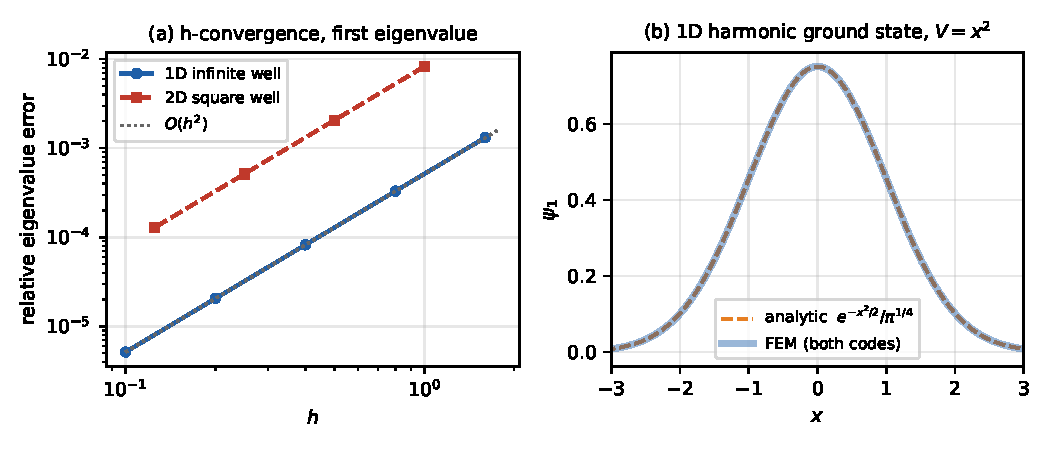
\includegraphics[width=\textwidth]{figuras/fig_convergencia.pdf}
\caption{(a) Relative error of the first eigenvalue against mesh size $h$ for
the 1D infinite well and the 2D square well, with the $\mathcal{O}(h^2)$
reference slope predicted by Corollary~\ref{cor:order}. (b) Ground state of the
1D harmonic oscillator, $V = x^2$: both implementations produce the analytic
Gaussian to within the line width.}
\label{fig:convergence}
\end{figure}

\subsection{Code-to-code verification}\label{sec:codetocode}

The strongest evidence in this study comes from comparing the two independent
implementations. Using identical meshes and potentials, and requesting the
lowest eigenvalue, the \textsf{Elmer} module and the Python code agree to
within $4\times10^{-13}$ in relative terms across all three spatial dimensions
(Table~\ref{tab:codetocode}). The last column of that table gives the normalised
residual $\|A_{ff}\boldsymbol{\psi} - E M_{ff}\boldsymbol{\psi}\| /
\|A_{ff}\boldsymbol{\psi}\|$ of the computed eigenpair. Both norms are Euclidean
and the eigenvector is normalised by
$\boldsymbol{\psi}^\top M_{ff}\boldsymbol{\psi} = 1$; dividing by
$\|A_{ff}\boldsymbol{\psi}\|$ makes the quantity dimensionless and independent of
the scaling of $A$, which is what allows rows with eigenvalues of very different
magnitude to be compared.

The level of agreement should be read with the conditioning of the problem in
mind. For the 1D well the first eigenvalue, $6.2\times10^{-3}$, is three orders
of magnitude smaller than $\|A_{ff}\| \approx 1/h = 6.25$, so the relative
accuracy attainable in $E_1$ is limited to roughly
$\varepsilon\,\|A_{ff}\|/E_1 \approx 10^{-12}$ in double precision, whatever
algorithm is used; the residual of $3.2\times10^{-11}$ in that row reflects the
same conditioning. For the 2D and 3D cases the eigenvector is well conditioned
and both the eigenvalue difference and the residual are at the $10^{-13}$ and
$10^{-14}$ levels respectively. We checked that three independent solution paths
for the 1D case (the in-framework dense solve, the exported sparse solve, and an
independent dense implementation written for this verification) differ among
themselves by up to $5\times10^{-12}$ in relative terms, which is the same
round-off scale.

\begin{table}[t]
\caption{Code-to-code verification: two independently written implementations on
identical meshes and potentials.}\label{tab:codetocode}
\begin{tabular}{@{}lccc c@{}}
\toprule
case & \textsf{Elmer} $E_1$ & Python $E_1$ & relative difference
& $\|A\psi - E M\psi\|/\|A\psi\|$ \\
\midrule
1D infinite well & $6.168583925347\times10^{-3}$ & $6.168583925345\times10^{-3}$ & $3.6\times10^{-13}$ & $3.2\times10^{-11}$ \\
2D harmonic & $1.028585384356000$ & $1.028585384356285$ & $2.8\times10^{-13}$ & $4.8\times10^{-14}$ \\
3D harmonic & $1.625507320678000$ & $1.625507320677697$ & $1.9\times10^{-13}$ & $1.1\times10^{-14}$ \\
\bottomrule
\end{tabular}
\end{table}

Because the two codes share no source code, use different mesh containers,
different assembly loops and different eigensolver libraries, agreement at this
level strongly constrains a broad class of implementation errors that comparison against
analytic solutions alone would not detect. The approach follows the spirit of
earlier cross-validation of independent codes in computational
physics \cite{paes2003} and is, in our assessment, the single most informative
result of the verification programme---available precisely because two
implementations were developed.

A related internal check is that solving the \emph{exported} matrices with the
sparse pipeline reproduces the dense in-framework solution (Table~\ref{tab:export}).
The twelve digits shown coincide, so the export introduces no error at the level
of the reported precision and the sparse route is a drop-in replacement for the
dense one. This is a statement about the two solution paths agreeing with each
other, not about either being exact: both solve the same discrete problem, and
both inherit whatever discretization error that problem carries.

\begin{table}[t]
\caption{The exported-matrix sparse route reproduces the in-framework dense
solution to all displayed digits.}\label{tab:export}
\begin{tabular}{@{}lcccc@{}}
\toprule
route & $E_1$ & $E_2$ & $E_3$ & $E_4$ \\
\midrule
in-framework (dense \texttt{DSYGV}) & $1.113644656498$ & $2.172208383659$ & $2.172208383659$ & $3.230772110820$ \\
exported $+$ sparse (ARPACK) & $1.113644656498$ & $2.172208383659$ & $2.172208383659$ & $3.230772110820$ \\
\bottomrule
\end{tabular}
\end{table}

\subsection{Structural consistency checks}\label{sec:structural}

Three checks require no external reference.

\textbf{Mass-orthonormality.} The computed eigenvectors must satisfy
$\boldsymbol{\psi}_i^\top M \boldsymbol{\psi}_j = \delta_{ij}$. We verified this
numerically; in the 2D case the largest deviation from the identity is
$3.1\times10^{-15}$, that is, at the level of double-precision round-off.

\textbf{Degeneracies.} Symmetry of the domain and potential implies degeneracies
of known multiplicity. The 2D isotropic harmonic oscillator on a square domain
must have a doubly degenerate first excited state; we obtain
$E_2 = E_3 = 2.043966018888$ to all displayed digits. In 3D the first excited
state is triply degenerate; we obtain $E_2 = E_3 = E_4 = 2.669307913349$.
Degeneracies are a strong test because they are destroyed if the assembly breaks
the symmetry---for instance through inconsistent element ordering or a
dimension-dependent quadrature error.

\textbf{Virial theorem.} For a harmonic potential the virial theorem
\cite{courant1953} requires
$\langle T\rangle = \langle V\rangle = E/2$. Multiplying \eqref{eq:strong} by
$\psi$ and integrating by parts gives
$\langle T\rangle = \int|\nabla\psi|^2\mathrm{d}\Omega$ and
$\langle V\rangle = \int V|\psi|^2\mathrm{d}\Omega$, so that
$E = \langle T\rangle + \langle V\rangle$ holds identically. Discretely, the
natural definitions are the quadratic forms of the assembled matrices,
$\langle T\rangle_h = \boldsymbol{\psi}^\top K\boldsymbol{\psi}$ and
$\langle V\rangle_h = \boldsymbol{\psi}^\top M_V\boldsymbol{\psi}$ with
$\boldsymbol{\psi}$ normalised by $\boldsymbol{\psi}^\top M\boldsymbol{\psi} = 1$;
then $E_h = \langle T\rangle_h + \langle V\rangle_h$ holds exactly by
construction, and only the ratio is a test. For the 1D harmonic ground state we
obtain
%
\begin{center}
\begin{tabular}{@{}rrrr@{}}
\toprule
$n$ & $\langle T\rangle_h$ & $\langle V\rangle_h$ & $\langle T\rangle_h/\langle V\rangle_h$ \\
\midrule
100  & $0.5000031$ & $0.5091573$ & $0.98202$ \\
200  & $0.5000002$ & $0.5022911$ & $0.99544$ \\
400  & $0.5000000$ & $0.5005729$ & $0.99886$ \\
800  & $0.5000000$ & $0.5001432$ & $0.99971$ \\
1600 & $0.5000000$ & $0.5000358$ & $0.99993$ \\
\bottomrule
\end{tabular}
\end{center}
%
The ratio approaches the exact value $1$ as $\mathcal{O}(h^2)$, while
$\langle T\rangle_h$ is already accurate to $10^{-8}$ at $n = 400$. The check is
notable because it relates the eigenvalue to the eigenfunction without invoking
the analytic form of the latter.

Two points about the finite box are worth separating. The identity
$E = \langle T\rangle + \langle V\rangle$ is an integration by parts whose
boundary term is $\psi\,\partial_n\psi$ on $\partial\Omega$, which vanishes
because $\psi = 0$ there; it therefore holds in a bounded box with no correction,
and the table confirms it ($E_h - \langle T\rangle_h - \langle V\rangle_h$ is at
round-off, $\sim10^{-14}$). The ratio $\langle T\rangle_h/\langle V\rangle_h$
is a different statement, derived from the scaling $x \mapsto \lambda x$, which
in a bounded box is not a symmetry of the problem. We checked numerically that
it is nevertheless independent of the box: at fixed $h = 0.25$ and $\alpha = 1$
the ratio equals $0.97221$ for every $L$ from $12$ to $28$, so the deviation
from $1$ is entirely the $\mathcal{O}(h^2)$ discretization error above and not a
truncation effect. The first row of the table, $0.98202$ at $n=100$, and the
value $0.97221$ at $h=0.25$ are consistent with this reading.

\textbf{Monotonicity.} By Theorem~\ref{thm:upper} the computed eigenvalues must
approach the exact ones from above under refinement. All sequences in
Table~\ref{tab:conv} satisfy this.

%%========================================================================
\section{Numerical experiments}\label{sec:experiments}
%%========================================================================

\subsection{Benchmark suite}

Unless stated otherwise, the timings and residuals reported below were obtained
on a single workstation with an Intel i7-1065G7 processor (4 physical cores,
8\,logical) and $31$\,GB of RAM, running Linux with \textsf{Elmer}~9.0 built
against \textsc{gfortran}~9.4.0, MKL and MUMPS, \textsf{Python}~3.10 with
\textsc{numpy}~1.24.4 and \textsc{scipy}~1.10.1. The eigensolver tolerances are
those of the libraries: LAPACK \texttt{DSYGV} uses its default, ARPACK is called
with \texttt{tol}$~=0$, so its stopping criterion is machine precision, and the
Elmer module uses the default of its own solver interface. The distributed runs
of Section~\ref{sec:decomposition} were made on a cluster node with 256 cores
and $251$\,GB of RAM. Timings are the wall-clock time of the eigensolution call
alone, excluding assembly; the sparse figures are the minimum of three
repetitions, and the dense figures a single run because of their cost. Absolute
times are properties of the hardware and are not transferable; the algorithmic
comparison is.

Seven cases were run to completion with the \textsf{Elmer} module, covering
smooth and non-smooth potentials, bound and quasi-bound states, and one- and
multidimensional geometries. Table~\ref{tab:cases} lists the four lowest
eigenvalues of each, together with the number of free degrees of freedom.
Figure~\ref{fig:potentials} shows the potentials and the computed levels.

\begin{table}[t]
\caption{Benchmark suite: four lowest eigenvalues for each case, in the unit
convention of \eqref{eq:strong}. The last column gives the number of free
degrees of freedom $n_f$ after elimination
(Proposition~\ref{prop:elim}).}\label{tab:cases}
\begin{tabular}{@{}lccccr@{}}
\toprule
case & $E_1$ & $E_2$ & $E_3$ & $E_4$ & $n_f$ \\
\midrule
1D infinite well    & $6.168584\times10^{-3}$ & $2.467531\times10^{-2}$ & $5.552310\times10^{-2}$ & $9.871683\times10^{-2}$ & 249 \\
1D harmonic         & $1.000572892$ & $3.001197697$ & $5.002447062$ & $7.004320695$ & 399 \\
1D Morse            & $-8.481033787$ & $-5.818565432$ & $-3.656064809$ & $-1.991029948$ & 399 \\
1D double well      & $0.224110514$ & $0.600028005$ & $1.274687373$ & $2.059803060$ & 399 \\
1D sinusoidal       & $-0.213200584$ & $-0.209442228$ & $0.285067468$ & $0.343455929$ & 399 \\
2D harmonic         & $1.028585384$ & $2.043966019$ & $2.043966019$ & $3.059346653$ & 1521 \\
3D harmonic         & $1.625507321$ & $2.669307913$ & $2.669307913$ & $2.669307913$ & 2197 \\
\bottomrule
\end{tabular}
\end{table}

Two features merit comment.

\textbf{The double well.} With a barrier separating two symmetric minima, the
two lowest states are split by tunnelling; we obtain $E_2 - E_1 = 0.376$, a
splitting that vanishes if the barrier is removed. The presence of a
\emph{finite} splitting is a sensitive indicator that the barrier region is
resolved and that the two wells are correctly coupled through it: a mesh too
coarse in the barrier overestimates it, and a symmetry-broken discretization can
suppress it artificially. Double-well structures of this kind are the standard
model for coupled quantum wells and for the tunnelling phenomena exploited in
resonant tunnelling devices \cite{wang2009}.

\textbf{The periodic potential.} The lowest two eigenvalues,
$-0.213200584$ and $-0.209442228$, lie just above the potential minimum
$V_{\min} = -0.5$ and are separated by only $3.8\times10^{-3}$, a near
degeneracy that is a property of this bounded interval and not, by itself, a band
structure: the computation imposes Dirichlet conditions and no quasi-momentum is
defined, so the levels are those of a finite segment of a periodic potential
rather than of a crystal. Establishing a band structure would require Bloch
conditions or a superlattice with many periods, and is outside the present scope.
Potentials of this type model superlattices and miniband structures
\cite{harrison2005}; for the computation of genuine band structures, where the
eigenproblem is again of the shift-and-invert type, see \cite{bandstruct2020}.

\begin{figure}[t]
\centering
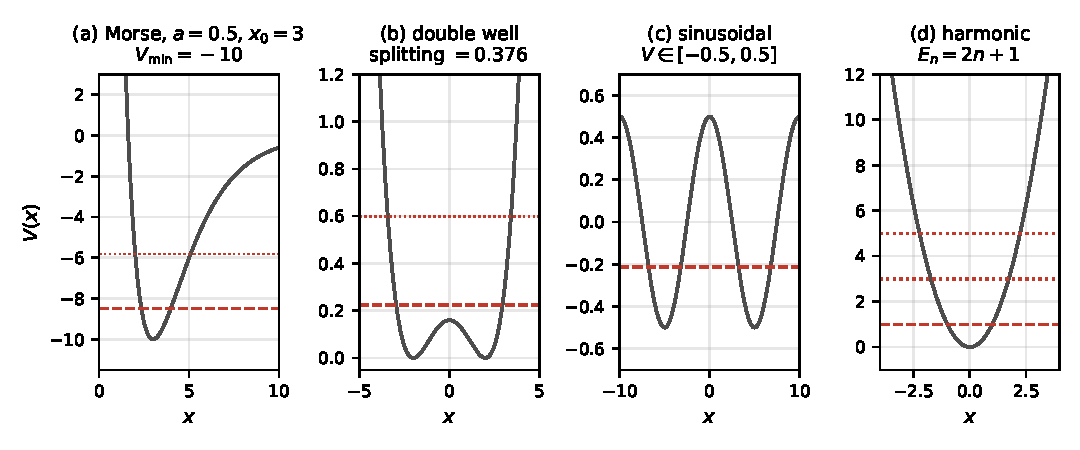
\includegraphics[width=\textwidth]{figuras/fig_potenciais.pdf}
\caption{Potentials of the 1D benchmark cases with the computed levels
(dashed and dotted lines): (a) Morse, $V_{\min} = -10$; (b) double well,
splitting $E_2 - E_1 = 0.376$; (c) sinusoidal,
$V \in [-0.5, 0.5]$; (d) harmonic, $E_n = 2n+1$.}
\label{fig:potentials}
\end{figure}

\subsection{Discretization error versus box truncation}\label{sec:truncation}

The harmonic cases deserve care, because two distinct error sources are easily
conflated there. The analytic eigenvalues $E_n = n + d/2$ in the convention of
\eqref{eq:strong} refer to an unbounded domain, whereas the computation imposes
$\psi = 0$ on the boundary of a finite box of side $L$. Both the finite box and
the finite mesh raise the computed eigenvalue, but by very different amounts; in
the cases considered here it is the mesh that dominates.

The truncation effect is negligible at these box sizes. By \eqref{eq:harmgs} the
analytic ground state is $\exp(-\sqrt{\alpha}\,r^2/2)$, so writing it as
$\exp(-r^2/2\sigma^2)$ the characteristic length is
$\sigma = \alpha^{-1/4}$---which for $\alpha = 1/4$ is $\sqrt{2}$ and
\emph{not} $\sqrt{\alpha} = 1/2$. On a centred box of side $L$ the amplitude at a
face is $\exp(-\sqrt{\alpha}\,L^2/8)$; for $\alpha = 1/4$ and $L = 12$ that is
$\exp(-9) \approx 1.2\times10^{-4}$ of the peak, so the exact solution very nearly
satisfies the Dirichlet condition already. \emph{If} one assumes the eigenvalue
perturbation to behave like the square of that amplitude, the estimate is
$10^{-8}$ or less; this is an order-of-magnitude heuristic and not a
demonstrated bound. The direct evidence is in Table~\ref{tab:box}, where the box
is varied at fixed mesh size.

That the discrepancy is instead a mesh effect is confirmed by refinement.
Table~\ref{tab:harm-conv} refines the 2D and 3D harmonic cases at fixed box size.
The errors decrease as $\mathcal{O}(h^2)$, in agreement with
Corollary~\ref{cor:order}, and the sequences converge to the \emph{unbounded}
values $1.0$ and $1.5$ rather than to any larger box eigenvalue. Refining the
mesh at fixed $L$ therefore recovers the analytic result, which would not occur
if the box were the controlling error.

The discrepancies quoted in Table~\ref{tab:cases}---$2.9\%$ in 2D at $h = 0.5$
and $8.4\%$ in 3D at $h = 0.857$---are thus discretization error at a
deliberately coarse mesh. The distinction is not merely semantic: reducing them
requires refining the mesh, not enlarging the box. Higher excited states, which
oscillate faster, are affected more strongly, and errors of $20$--$40\%$ appear
in the fourth eigenvalue at these mesh sizes. Box dimensions and mesh sizes are
therefore reported explicitly (Appendix~\ref{app:cases}).

A second, independent check separates the two effects by varying the box at
\emph{fixed} mesh size. Table~\ref{tab:box} reports the first eigenvalue of the
2D and 3D harmonic cases for a sequence of boxes, with $h$ held at $0.5$ and
$1.0$ respectively. In 2D the value is constant to twelve significant
digits from $L=16$ onwards. In 3D, where the fixed mesh is much coarser, it is
constant to nine significant digits from $L=12$ onwards; the coarser plateau
reflects the larger discretization error and not a larger truncation effect,
since the box is already several times the characteristic length of the
ground state. In both cases the offset from the unbounded analytic value ($1$
and $1.5$) is a pure discretization error at the fixed mesh size---$2.9\times
10^{-2}$ at $h=0.5$ in 2D and $1.7\times10^{-1}$ at $h=1.0$ in 3D---and does
not shrink as the box grows. Truncation is therefore below the resolution of
the computation over the range tested, which is the direct evidence that the
discrepancies of Table~\ref{tab:cases} must be attributed to the mesh. The
statement is limited to the boxes and mesh sizes reported: a box smaller than
$L=12$ in 3D does show a truncation error, as the first row of
Table~\ref{tab:box} makes plain.

\begin{table}[t]
\caption{Domain-size study at \emph{fixed} mesh size. Once the box is large
enough the first eigenvalue stops changing, while the offset from the unbounded
value does not: the offset is discretization, not truncation. The variations in
the last digits are round-off.}\label{tab:box}
\begin{tabular}{@{}lrrrr@{}}
\toprule
\multicolumn{5}{@{}l}{2D harmonic, $h = 0.5$, $\alpha=1/4$, unbounded $E_1 = 1$} \\
$L$ & 12 & 16 & 28 & 40 \\
$n_f$ & 529 & 961 & 3\,025 & 6\,241 \\
$E_1$ & $1.028585446$ & $1.028585384$ & $1.028585384$ & $1.028585384$ \\
\midrule
\multicolumn{5}{@{}l}{3D harmonic, $h = 1.0$, $\alpha=1/4$, unbounded $E_1 = 1.5$} \\
$L$ & 6 & 9 & 12 & 18 \\
$n_f$ & 125 & 512 & 1\,331 & 4\,913 \\
$E_1$ & $1.737955701$ & $1.670595303$ & $1.670466988$ & $1.670466985$ \\
$\Delta E_1$ & --- & $6.7\times10^{-2}$ & $1.3\times10^{-4}$ & $3\times10^{-9}$ \\
\bottomrule
\end{tabular}
\end{table}

\begin{table}[t]
\caption{Refinement of the harmonic cases at fixed box size. Both sequences
converge to the \emph{unbounded} analytic values rather than to a larger box
eigenvalue, showing that the leading error is discretization and not box
truncation. The last column gives the order observed between consecutive
refinements, $\log(e_i/e_{i+1})/\log(h_i/h_{i+1})$, computed from the relative
errors $e_i$ (Remark~\ref{rem:order}).}\label{tab:harm-conv}
\begin{tabular}{@{}lrrrrr@{}}
\toprule
case & $n$ & $h$ & $E_1$ & relative error & observed order \\
\midrule
2D, $L=20$, $\alpha=1/4$ & 20 & $1.000$ & $1.113645$ & $1.14\times10^{-1}$ & --- \\
                         & 40 & $0.500$ & $1.028585$ & $2.86\times10^{-2}$ & $1.99$ \\
                         & 60 & $0.333$ & $1.012719$ & $1.27\times10^{-2}$ & $2.00$ \\
                         & 80 & $0.250$ & $1.007158$ & $7.16\times10^{-3}$ & $2.00$ \\
\midrule
3D, $L=12$, $\alpha=1/4$ & 10 & $1.200$ & $1.744630$ & $1.63\times10^{-1}$ & --- \\
                         & 14 & $0.857$ & $1.625507$ & $8.37\times10^{-2}$ & $1.98$ \\
                         & 18 & $0.667$ & $1.576105$ & $5.07\times10^{-2}$ & $1.99$ \\
                         & 20 & $0.600$ & $1.561688$ & $4.11\times10^{-2}$ & $1.99$ \\
\bottomrule
\end{tabular}
\end{table}

\begin{remark}[Quadrature of the potential term]\label{rem:quadrature}
The error constant depends on how the potential enters the weighted mass matrix
\eqref{eq:local}. Both implementations assemble $\int N_i V_h N_j$, that is, they
use the \emph{interpolant} $V_h$ of $V$ in the finite element space rather than
evaluating $V$ exactly at the quadrature points---which is the natural convention
in a general finite element code, where the potential is supplied as a nodal
field. For the quadratic potentials considered here this introduces an additional
$\mathcal{O}(h^2)$ contribution; it does not change the order of convergence but
does increase the constant. Recomputing the 1D harmonic case ($L = 20$, $400$
elements) with $V$ evaluated exactly at the quadrature points raises the accuracy
of the first eigenvalue from $1.000572892$ to $1.000156243$, against the exact
value $1$. We retain the interpolant convention and record the difference here.
\end{remark}

\subsection{Eigensolution performance}\label{sec:performance}

Table~\ref{tab:performance} and Figure~\ref{fig:performance} compare the dense
and sparse strategies on the 2D harmonic case, holding the mesh and the number
of requested eigenpairs ($k = 4$) fixed. The discretization is identical in all
rows; only the solver changes. The first column gives the dimension of the
reduced matrices, that is, the number of free degrees of freedom after the
elimination of Proposition~\ref{prop:elim}; for a structured mesh of
$n\times n$ elements on a square with Dirichlet data on the whole boundary this
is $(n-1)^2$. The measurements were taken on a workstation with $31$\,GB of
memory, and were reproduced on a cluster node; the absolute times differ between
the two machines, but the algorithmic behaviour is the same.

\begin{table}[t]
\caption{Eigensolution time for the 2D harmonic case, $k = 4$, as a function of
the number of free degrees of freedom $n_f$. Identical matrices in both columns.
The last row is not merely slow in dense arithmetic but exceeds the memory of the
workstation used ($31$\,GB): at $24\,n_f^2$ it requires $37.6$\,GB, cf.\
\eqref{eq:densemem}. On a large-memory node it would fit, but the sparse route
makes the question moot. In the first row the sparse time is below the resolution
of the timer, so no speed-up is quoted there and none is annotated in
Figure~\ref{fig:performance}.}\label{tab:performance}
\begin{tabular}{@{}rrrrr@{}}
\toprule
$n_f$ & dense \texttt{DSYGV} (s) & sparse ARPACK (s) & speed-up & dense memory \\
\midrule
361   & $0.01$   & $<0.01$ & --- & $3.1$\,MB \\
1\,521 & $0.58$   & $0.01$  & $58\times$ & $55.5$\,MB \\
6\,241 & $41.06$  & $0.05$  & $821\times$ & $935$\,MB \\
14\,161 & $491.60$ & $0.12$  & $4097\times$ & $4.81$\,GB \\
39\,601 & infeasible ($37.6$\,GB) & $0.41$ & --- & $37.6$\,GB \\
\bottomrule
\end{tabular}
\end{table}

The measured speed-up grows faster than linearly. A factor $70$ in speed-up for
a factor $9.3$ in problem size would be consistent with an $\mathcal{O}(n_f^2)$
ratio, but with three interior points we do not claim to have identified an
asymptotic exponent; what the data establish is the behaviour---sub-quadratic
cost in $n_f$ against cubic for the dense route---and the resulting crossover,
not a fitted law
$T_{\text{dense}}/T_{\text{sparse}}$. The comparison at the largest case is not a
timing comparison at all: the dense route cannot be run. This is the practical
argument for the sparse strategy---it is not merely faster, it extends the
accessible problem class.

\begin{figure}[t]
\centering
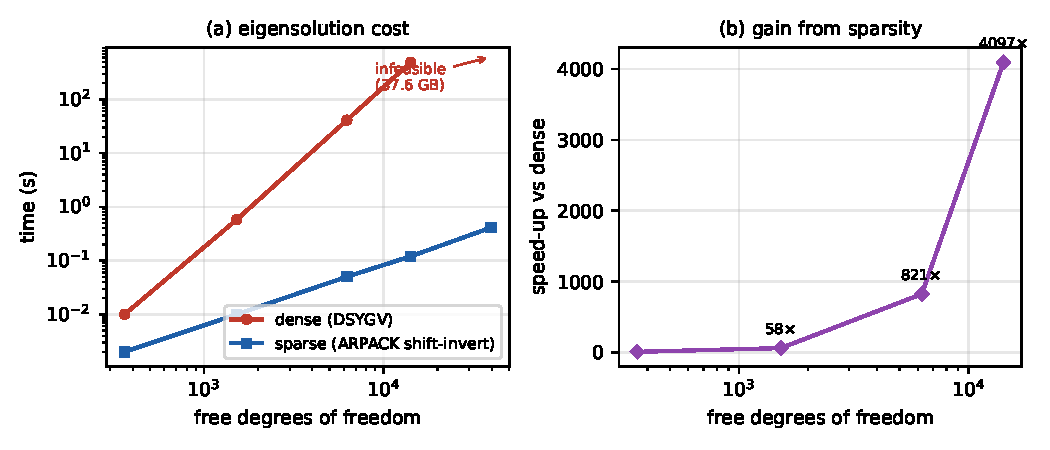
\includegraphics[width=\textwidth]{figuras/fig_desempenho.pdf}
\caption{(a) Eigensolution time against problem size for the dense and sparse
strategies, on identical matrices. (b) Speed-up of the sparse strategy over the
dense one, with measured values annotated.}
\label{fig:performance}
\end{figure}

Thread-level parallelism does not substitute for the algorithmic change.
Enabling multithreaded BLAS in the sparse solve at $n_f = 39601$ we obtain
$0.84$\,s with one thread, and $1.10$, $1.10$ and $2.25$\,s with two, four and
eight threads respectively (minimum of three repetitions). Threading therefore
gives no speed-up at all here---it degrades the result, since the extra workers
contend for the same memory bandwidth while the sparse factorization itself
remains sequential. This reinforces the point of
Section~\ref{sec:strategies}: the gain must come from the algorithm, not from
the hardware.

\subsection{Behaviour under domain decomposition}\label{sec:decomposition}

We report a negative result, because it defines the boundary of applicability of
the in-framework solver and motivates the second route discussed in
Section~\ref{sec:routes}.

The \textsf{Elmer} module is \emph{not} MPI-aware, and two distinct problems
arise when it is run under \texttt{mpirun -np} with more than one process.

The first is a defect in \textsf{Elmer} 9.0 independent of our module. The
routine that builds the mesh path for a partitioned run issues only a
\emph{warning}---not a fatal error---when the partition header file is absent,
and returns a null pointer. The caller dereferences the result \emph{before} the
associated-pointer check a few lines later, producing a segmentation fault. A
controlled A/B test confirms the diagnosis: the same binary segfaults at
\texttt{-np 2} without the partition directory and exits cleanly with it
present.

The second problem is specific to the solver and more serious. Even when the
mesh \emph{is} partitioned, the module assembles dense \emph{local} matrices on
each rank. The assembly loop uses rank-local element and node counts, so each
rank solves a different, smaller problem and the results are simply wrong. On a
small test mesh, where the serial result can be checked by hand, we obtain:

\begin{center}
\begin{tabular}{@{}lcc@{}}
\toprule
 & serial & \texttt{-np 2} \\
\midrule
free degrees of freedom & 59 & 29 \emph{per rank} \\
$E_1$ & $1.025415149101$ & $3.052806819296$ \\
\bottomrule
\end{tabular}
\end{center}

\noindent
The failure is silent---the run completes and reports eigenvalues---which makes
it more dangerous than a crash. We therefore do not recommend distributed
execution of the in-framework solver in its present form. The correct fix, a
solver with native parallel assembly following the pattern of the existing
\textsf{Elmer} wavefunction solver, remains future work.

%%========================================================================
\section{Discussion}\label{sec:discussion}
%%========================================================================

\subsection{Two routes and their crossover}\label{sec:routes}

The results above suggest a practical division of labour rather than a single
recommended strategy.

\textbf{In-framework route (dense, serial).} Up to roughly $10^4$ free degrees of
freedom---which covers a wide range of one- and two-dimensional quantum-well and
quantum-dot calculations at engineering accuracy---the dense in-framework solver
is the simpler choice. It requires no matrix export and keeps the entire
workflow inside the finite element framework, including post-processing. The
$n_f = 6561$ case solves in $41$\,s, acceptable for interactive use.

\textbf{Export route (sparse, parallel-capable).} Beyond that size, and whenever
several eigenpairs are needed or the mesh must be refined, the matrices should
be exported and solved externally. This route reproduces the dense result
exactly (Table~\ref{tab:export}), reduces storage from $\mathcal{O}(n_f^2)$ to
$\mathcal{O}(\mathrm{nnz})$, and---given a parallel sparse direct
factorization---scales across nodes. The exported matrices are the \emph{same}
matrices: the route is a change of linear algebra, not of discretization, so the
two solve the same discrete problem and agree to the reported precision
(Table~\ref{tab:export}). They are not required to agree bit for bit, since two
different algorithms on the same matrices need not round identically; the choice
between them is one of computational resources.

The crossover follows from \eqref{eq:densemem}, and the factor matters. If only
the irreducible two matrices are retained, $16n_f^2$ bytes are needed and the
dense route becomes impractical at $n_f \sim 10^4$ for a $1.6$\,GB budget and
$n_f \sim 4\times10^4$ for $25$\,GB. The implementation measured here holds
three matrices, so the relevant coefficient is $24n_f^2$ and the same budgets
are reached earlier, at $n_f \sim 8\times10^3$ and $n_f \sim 3.2\times10^4$.
Both figures are estimates from the storage model alone; they take no account of
the workspace the eigensolver itself allocates, which only makes the dense route
less attractive.

\subsection{Limitations}\label{sec:limitations}

\textbf{Separable potentials.} The component-wise convention of
Section~\ref{sec:potential} restricts the module to potentials of the form
$\sum_k V_k(x_k)$. Non-separable potentials---a Coulomb term, or the $1/r$
inter-electronic interaction used in quantum-dot models \cite{caruso2019}---would
require extending the expression interface, not the solver core. Coupling to a
self-consistent Poisson equation, as in the Schr\"odinger--Poisson problem
\cite{wang2009,coos2014}, is likewise outside the present scope, as is the
treatment of open boundary conditions and polar geometries \cite{polar2020}.
For time-dependent and nonlinear formulations, which lie outside the scope
considered here, we refer to \cite{sav2023,liu2020}.

\textbf{No parallel in-framework solver.} As documented in
Section~\ref{sec:decomposition}, the module is serial; parallelism is obtained
through the export route. The scaling of that route is limited by the
availability of a parallel sparse direct factorization in the deployed PETSc
build; on the installation used here, PETSc was configured without a parallel
LU, so the shift-and-invert step could not be distributed and the driver was
confined to one process. The driver is complete and verified at one process;
only the linear-algebra backend is missing. We regard this as a deployment issue
rather than a methodological limitation, but it does mean we cannot report
parallel scaling numbers, and we prefer to say so.

\textbf{Coarse meshes for the confined cases.} As shown in
Section~\ref{sec:truncation}, the discrepancies in the harmonic cases are
discretization error, not box truncation: the boxes are large enough that the
truncation contribution is several orders of magnitude smaller. Reducing those
discrepancies therefore requires mesh refinement, and the meshes used for the 2D
and 3D harmonic cases are deliberately coarse. For potentials that decay slowly,
or for boxes chosen too small, truncation would become the leading error and
would then have to be separated from the discretization error.

\textbf{Only the ground state is written to file.} The module returns all
requested eigenvalues but writes only the first eigenfunction to the field
database, so the standard output modules produce a single mode per run.

\subsection{On the nature of the contribution}

We state plainly that the work introduces no new numerical algorithm. The
elements are standard multilinear Lagrange elements, the quadrature is standard
Gauss--Legendre, the eigensolvers are LAPACK, ARPACK and SLEPc, and the weak
form is textbook. Because the novelty is not algorithmic, we prefer to state
explicitly what the paper does contribute, so that the reader can weigh each
item against the alternatives.

\textbf{Reusable software.} A dimension-generic solver for
\eqref{eq:schrodinger} distributed as a module of \textsf{Elmer}, with all seven
benchmark cases, their meshes, their input files and a container definition that
reproduces the environment. The module did not previously exist in that
framework, and the packaging is intended so that a third party can reproduce
every number in this paper without contacting the authors.

\textbf{Corrected analysis for a common pitfall.} Section~\ref{sec:dirichlet}
shows, with numerical evidence, that the diagonal-shift treatment of Dirichlet
data used routinely for source problems is invalid here, and distinguishes the
two variants of that recipe and their different failure modes. The proof of
Proposition~\ref{prop:elim} is written in terms of the variational restriction,
which is the form that survives scrutiny; the naive block-matrix argument, as
Remark~\ref{rem:elimrows} shows, happens to hold for exponentially decaying
eigenfunctions and fails for the infinite well.

\textbf{Scoped theoretical statements.} Theorems~\ref{thm:upper}
and~\ref{thm:conv} are stated with the hypotheses they actually require.
Remark~\ref{rem:upperscope} records that the upper-bound property is not
preserved by the nodal interpolation of the potential for non-convex $V$, and
that it is therefore verified numerically rather than assumed;
Remark~\ref{rem:order} separates the theoretical convergence order from the
order observed on a particular sequence of meshes.

\textbf{Quantified comparison.} Dense and sparse eigensolution strategies are
compared on identical matrices, with a cost model that separates assembly,
factorization, iteration and solver overhead
(Section~\ref{sec:costmodel}), and the crossover between the two routes is
estimated. The distributed route is analysed and its present limitations
documented; it is not benchmarked, and we say so.

\textbf{A verification programme.} Four independent checks---analytic
benchmarks, code-to-code comparison of two independently written
implementations, structural invariants, and convergence orders---each reporting
residuals and conditioning where relevant. We consider the code-to-code
comparison the strongest of the four, and
Section~\ref{sec:codetocode} explains why its apparent agreement is limited by
the conditioning of the problem rather than by the quality of either code.

We believe this profile is representative of a useful class of work in
computational science: not new mathematics, but verified, characterised and
reusable numerical software, accompanied by analysis that is correct as stated
rather than correct by accident.

%%========================================================================
\section{Conclusions}\label{sec:conclusions}
%%========================================================================

We have presented a finite element framework for the stationary Schr\"odinger
eigenvalue problem, implemented independently in two codes and verified in four
ways. The main findings are the following.

\begin{enumerate}
  \item The generalized symmetric eigenproblem $A\psi = EM\psi$ with
        $A = K + M_V$ is solved accurately by multilinear finite elements in one,
        two and three dimensions. Where the discrete form is the exact
        restriction of the continuous one, the conforming approximation yields
        eigenvalues that are upper bounds for the exact ones
        (Theorem~\ref{thm:upper}); the implementation's nodal interpolation of
        the potential preserves that property for convex $V$ and is checked
        numerically for the others (Remark~\ref{rem:upperscope}). The eigenvalue
        error obeys the classical $\mathcal{O}(h^{2s})$ estimate
        of Theorem~\ref{thm:conv}; the predicted $\mathcal{O}(h^2)$ order is
        confirmed numerically over four refinements in 1D and four in 2D.
  \item Elimination of the constrained degrees of freedom reproduces the
        constrained spectrum exactly (Proposition~\ref{prop:elim}), whereas the
        common diagonal-shift treatment introduces spurious eigenvalues at
        $E = 1$.
  \item Two independently written implementations---a Fortran module for
        \textsf{Elmer} and a Python reference code---agree to approximately
        $4\times10^{-13}$ on identical problems. This code-to-code comparison is the
        strongest single verification result available and is strictly more
        informative than comparison against analytic solutions alone.
  \item The choice of eigensolution strategy dominates the computational cost.
        Replacing a dense solve by sparse shift-and-invert Arnoldi iteration
        yields speed-ups from $58\times$ to $4097\times$ and reduces storage from
        $\mathcal{O}(n_f^2)$ to $\mathcal{O}(\mathrm{nnz})$, extending the
        accessible problem size from roughly $10^4$ to at least
        $4\times10^4$ degrees of freedom on the same hardware, in agreement with
        the cost model \eqref{eq:costmodel}.
  \item The in-framework solver is not suitable for distributed execution in its
        current form: two distinct failure modes were identified and are
        documented here. Exporting the matrices and solving them with a sparse
        distributed library can be made correct; whether it is faster on a given
        problem depends on the availability of a parallel sparse direct solver,
        which we did not have and therefore did not measure.
  \item Structural checks requiring no external reference---expected
        degeneracies, mass-orthonormality, the virial theorem, and monotonicity
        of the eigenvalues under refinement---are inexpensive and detect errors
        that analytic comparisons at a single resolution can miss.
\end{enumerate}

Future work will address native parallel assembly in the solver module, the
extension to non-separable and self-consistent potentials, and the integration
of the solver into a multiphysics environment where the potential itself is
produced by a coupled transport or electromagnetic calculation. Coupled finite
element formulations of exactly this kind, in which fluid and electromagnetic
fields are solved within a single model, have been developed for
magnetohydrodynamic flows \cite{fonseca2021}; adding a quantum-mechanical
eigenproblem to such a framework is the natural next step.

%%========================================================================
\backmatter
%%========================================================================

\bmhead{Supplementary information}

The following material accompanies this article: the complete source of the
\textsf{Elmer} solver module and of the Python reference implementation; the
seven benchmark cases with their mesh definition files; step-by-step tutorials
for each case following the structure of the official \textsf{Elmer}
documentation; and a container definition that reproduces the software
environment used for all reported results.

\bmhead{Acknowledgements}

The author thanks CSC -- IT Center for Science for developing and maintaining
\textsf{Elmer} as open-source software. Computational resources were provided by
the high-performance computing cluster of the Federal University of Par\'a.

%%========================================================================
\section*{Declarations}
%%========================================================================

\begin{itemize}
\item Funding: The Article Processing Charge (APC) of this future publication
      will be funded by the Coordination for the Improvement of Higher Education
      Personnel --- CAPES (ROR identifier: 00x0ma614). For the purpose of open
      access, the author has applied a Creative Commons CC BY licence to any
      accepted version of the article. This is the acknowledgement text required
      by Art.~9, item~X of CAPES Ordinance no.~224/2026.
\item Conflict of interest: The author declares that he has no conflict of
      interest.
\item Ethics approval: Not applicable.
\item Consent to participate: Not applicable.
\item Consent for publication: Not applicable.
\item Data availability: The mesh files and solver input files for all seven
      benchmark cases are included as supplementary material.
\item Materials availability: Not applicable.
\item Code availability: Both implementations are open source, together with the
      case definitions, the container definition and the tutorials:
      \emph{[repository URL to be inserted]}.
\item Author contribution: The author is the sole contributor to this work:
      formulation, implementation, verification, and writing of the manuscript.
\end{itemize}

%%========================================================================
\begin{appendices}
%%========================================================================

\section{Analytic reference solutions}\label{app:analytic}

All expressions are stated in the unit convention of \eqref{eq:strong}, that is,
with a unit coefficient on the Laplacian. The relation to physical units is
given in Section~\ref{sec:units}.

\textbf{Infinite well, one dimension.} For $V = 0$ on $[-L/2, L/2]$ with
$\psi(\pm L/2) = 0$, $E_n = (n\pi/L)^2$ for $n = 1, 2, \dots$

\textbf{Infinite box, $d$ dimensions.} For a $d$-dimensional box of side $L$ with
homogeneous Dirichlet conditions on all faces,
$E_{n_1\dots n_d} = (\pi^2/L^2)\sum_{k=1}^{d} n_k^2$.

\textbf{Isotropic harmonic oscillator.} For $V = \alpha r^2$ with
$r^2 = \sum_k x_k^2$ the problem separates and
%
\begin{equation}\label{eq:harmlevels}
  E_N = (2N + d)\sqrt{\alpha} , \qquad N = 0, 1, 2, \dots ,
\end{equation}
%
where $N$ is the \emph{total} excitation number and $E_0 = d\sqrt{\alpha}$ is the
ground-state energy. The normalised ground state is
%
\begin{equation}\label{eq:harmgs}
  \psi_0(\mathbf{r}) = \left(\frac{\sqrt{\alpha}}{\pi}\right)^{d/4}
  \exp\!\left(-\frac{\sqrt{\alpha}}{2}\,r^2\right),
\end{equation}
%
which follows from $\int_{\mathbb{R}}\exp(-ax^2)\mathrm{d}x = \sqrt{\pi/a}$ with
$a = \sqrt{\alpha}$ applied in each coordinate. The prefactor is
$(\sqrt{\alpha}/\pi)^{d/4}$ and \emph{not} $(\alpha/\pi)^{d/4}$; the two coincide
only at $\alpha = 1$, which is why the case plotted in
Figure~\ref{fig:potentials} does not distinguish them, whereas the 2D and 3D
benchmark cases use $\alpha = 1/4$ and do.

The multiplicity of the level with total excitation $N$ is
%
\begin{equation}
  g_N = \binom{N + d - 1}{d - 1},
\end{equation}
%
so the first excited level, $N = 1$ and $E = d + 2$ for $\alpha = 1$, has
multiplicity $d$---doubly degenerate in 2D and triply degenerate in 3D. This is
the property used as a symmetry check in Section~\ref{sec:structural}, and it is
confirmed by the $2.669307913$ eigenvalue appearing three times in the 3D row of
Table~\ref{tab:cases}. The multiplicity $d(d+1)/2$ belongs to the \emph{second}
excited level, $N = 2$, $E = d + 4$, and not to the first.

\textbf{Morse potential.} For
$V(x) = D_e(1 - e^{-a(x-x_0)})^2 - D_e$ the spectrum consists of a finite number
of bound states, with
%
\begin{equation}\label{eq:morse}
  E_\nu = 2a\sqrt{D_e}\,(\nu + \tfrac12) - a^2(\nu + \tfrac12)^2 - D_e ,
  \qquad \nu = 0, 1, \dots
\end{equation}
%
for the full line. The case used here is $D_e = 10$, $a = 0.5$ and $x_0 = 3$,
on the truncated domain $[0,10]$; at $x = 0$ the potential has already reached
$111.2$, so the left wall is effectively infinite, while at $x = 10$ it stands at
$-0.595$. We use this as a quantitative check
(Section~\ref{sec:verification}). Because \eqref{eq:morse} holds on the full
line and the computation is performed on $[0,10]$, the comparison carries a
truncation contribution as well as a discretization one. On this mesh and box
the computed levels lie above the closed-form values by
$3.3\times10^{-4}$ to $3.5\times10^{-3}$ in absolute terms. \emph{Relative} to
each level the deviations are $3.9\times10^{-5}$, $8.9\times10^{-5}$,
$2.0\times10^{-4}$ and $1.7\times10^{-3}$ for $\nu = 0,1,2,3$: the range is
$4\times10^{-5}$ to $1.7\times10^{-3}$, the largest value arising in the
$\nu = 3$ level because it is the smallest in magnitude, not because it is the
worst resolved. A Richardson extrapolation of the mesh sequence agrees with the
closed-form values to $10^{-8}$, so the bulk of that difference is the
discretization at $n=400$ and the truncation is the smaller part.

\section{Benchmark case parameters}\label{app:cases}

\begin{table}[h]
\caption{Parameters of the benchmark cases. All meshes are structured and were
generated with \textsf{Gmsh}.}\label{tab:params}
\begin{tabular}{@{}llllr@{}}
\toprule
case & dimension & domain & potential & elements \\
\midrule
1D infinite well & 1 & $[-20, 20]$ & $V = 0$ & 250 \\
1D harmonic      & 1 & $[-10, 10]$ & $V = x^2$ & 400 \\
1D Morse         & 1 & $[0, 10]$   & $V = 10(e^{-2a(x-x_0)} - 2e^{-a(x-x_0)})$, $a = 0.5$, $x_0 = 3$ & 400 \\
1D double well   & 1 & $[-10, 10]$ & $V = 0.01(x^2 - 4)^2$ & 400 \\
1D sinusoidal    & 1 & $[-10, 10]$ & $V = 0.5\cos(2\pi x/10)$ & 400 \\
2D harmonic      & 2 & $[-10,10]^2$ & $V = 0.25(x^2 + y^2)$ & $40\times40$ \\
3D harmonic      & 3 & $[-6,6]^3$  & $V = 0.25(x^2 + y^2 + z^2)$ & $14^3$ \\
\bottomrule
\end{tabular}
\end{table}

\noindent
In all cases homogeneous Dirichlet conditions are imposed on the whole boundary.
The potentials of the 2D and 3D harmonic cases are specified through the
component-wise convention of Section~\ref{sec:potential}.

\end{appendices}

%%========================================================================
\bibliography{artigo_JSC}
%%========================================================================

\end{document}
